%!TEX TS-program = pdflatex
%!TEX root = tesi.tex
%!TEX encoding = UTF-8 Unicode

%\begin{tabular}{p{0.5\textwidth} p{0.4\textwidth}}
%    \vspace{0pt} 
%    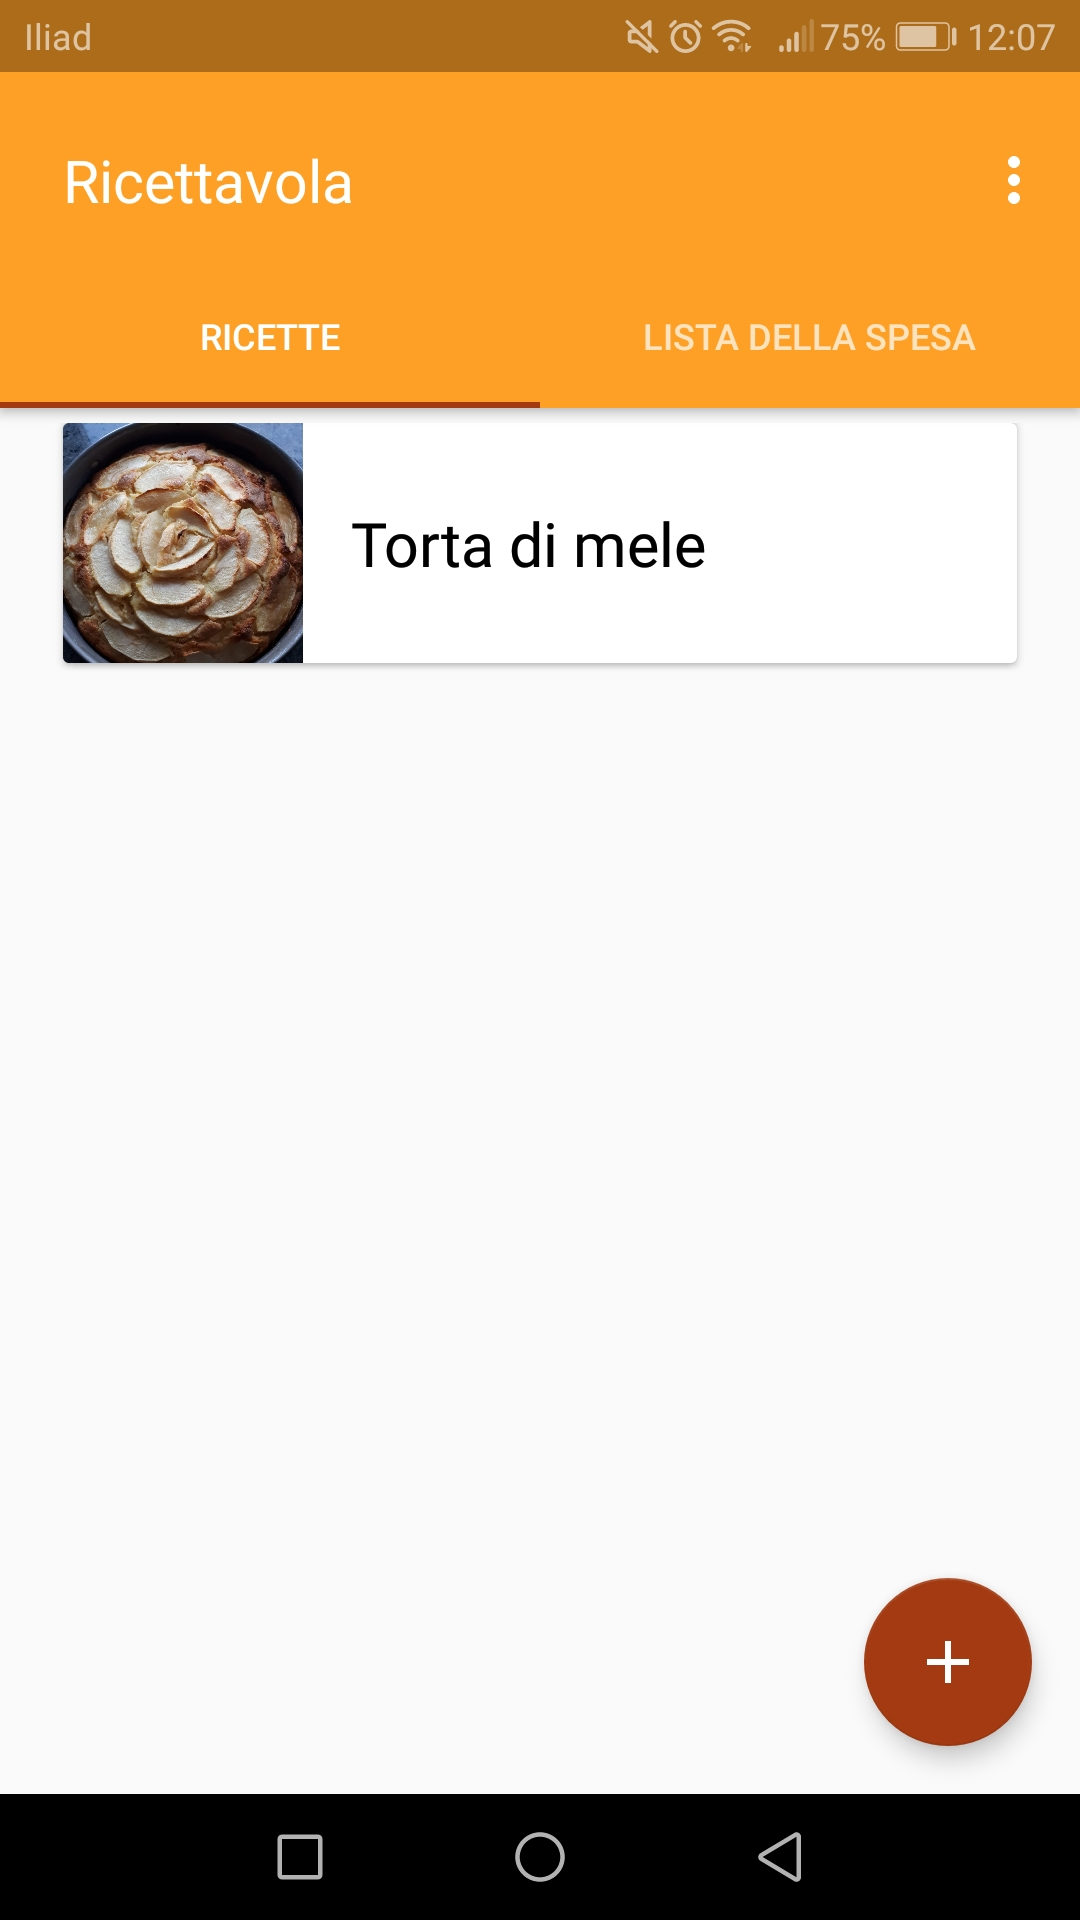
\includegraphics[width=0.5\textwidth]{definitivo/main}
%    & 
%    \vspace{0pt}
%    La schermata principale si presenta come quella progettata durante la prototipizzazione.
%    I tab permettono di spostarti tra le ricette e la lista della spesa.
%    \\
%\end{tabular}



\section{Risultato}
Ora verranno illustrate le schermate dell'applicazione implementata con Android Studio.

In figura \ref{fig:def_main} è riportata le schermata principale.
Si può notare che la lista delle ricette non presenta differenze rispetto al prototipo a bassa fedeltà.
La lista della spesa invece non è suddivisa per ricette, spetterà all'utente assicurarsi se gli ingredienti ripetuti sono stati ripetuti volutamente o per errore.
Gli ingredienti possono essere selezionati o deselezionati.

\begin{figure}[ht]
  \begin{center}
    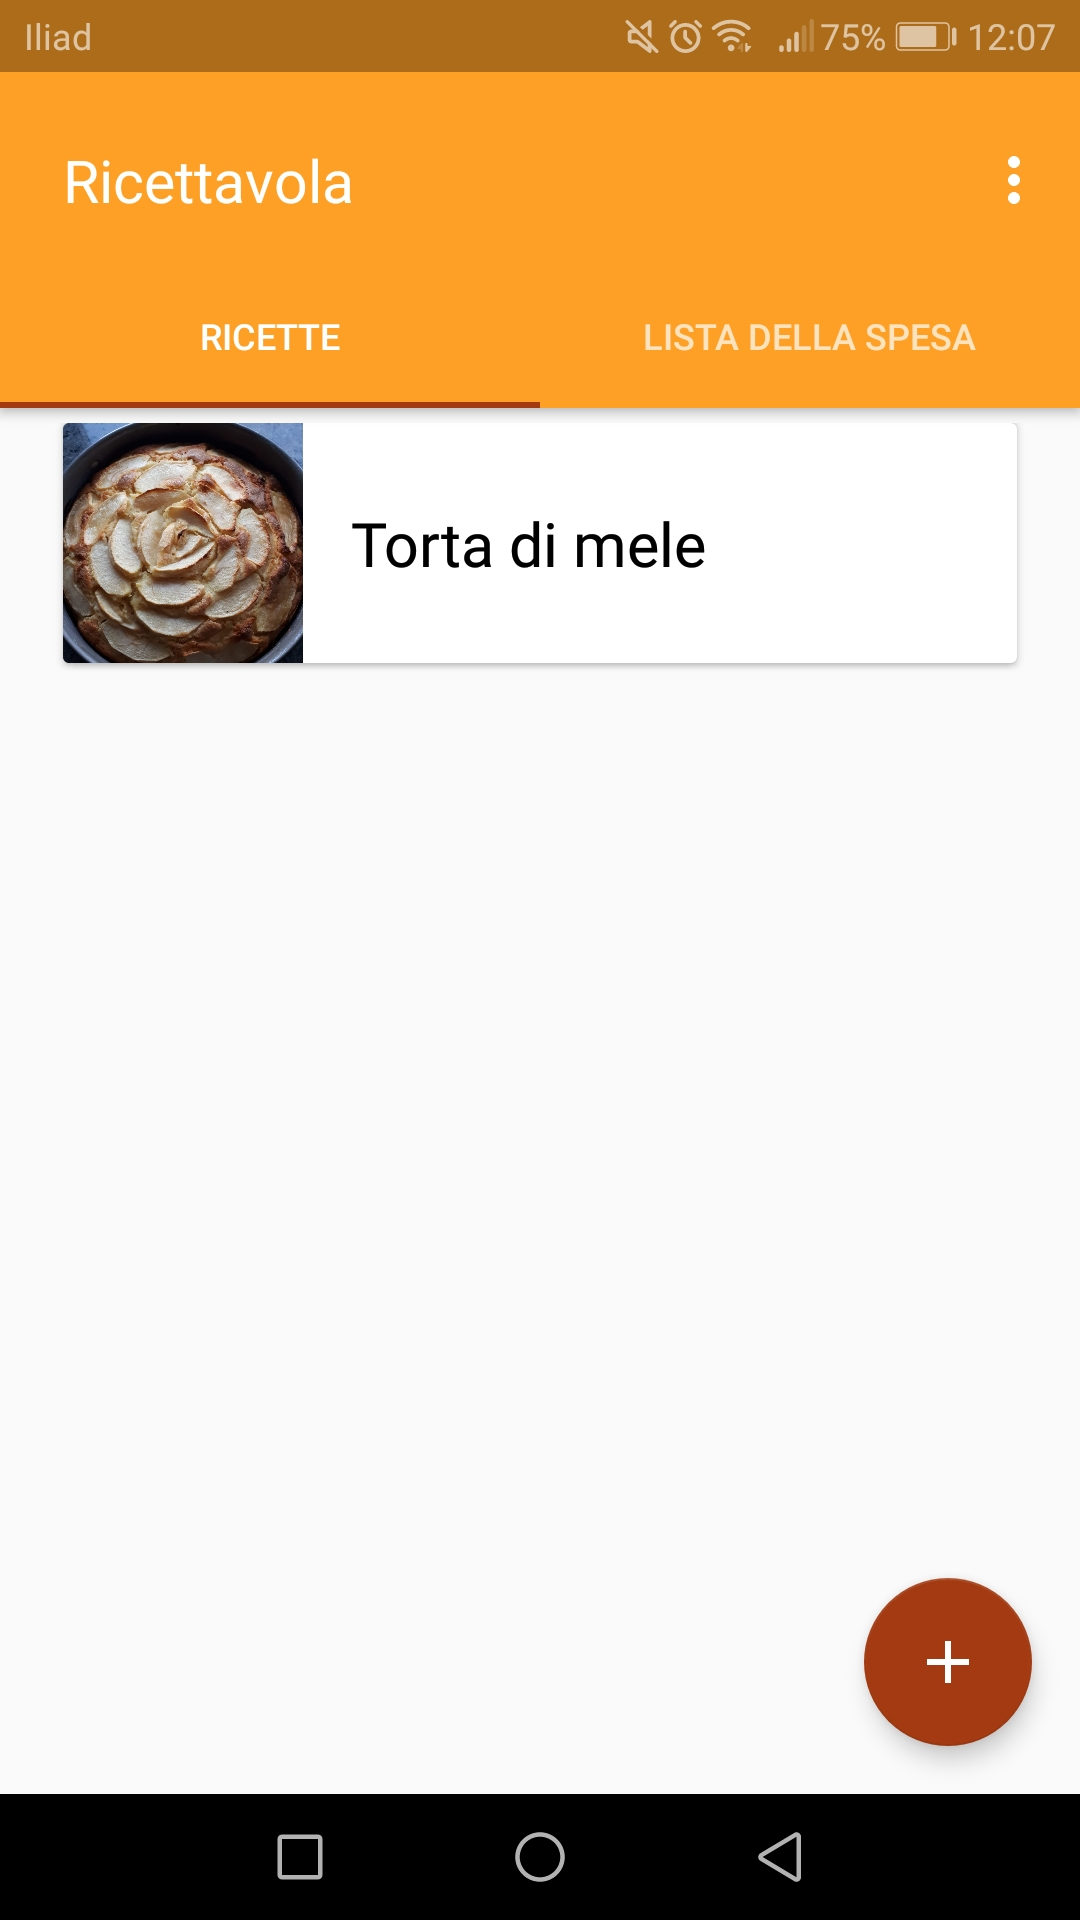
\includegraphics[width=0.49\textwidth]{definitivo/main}
    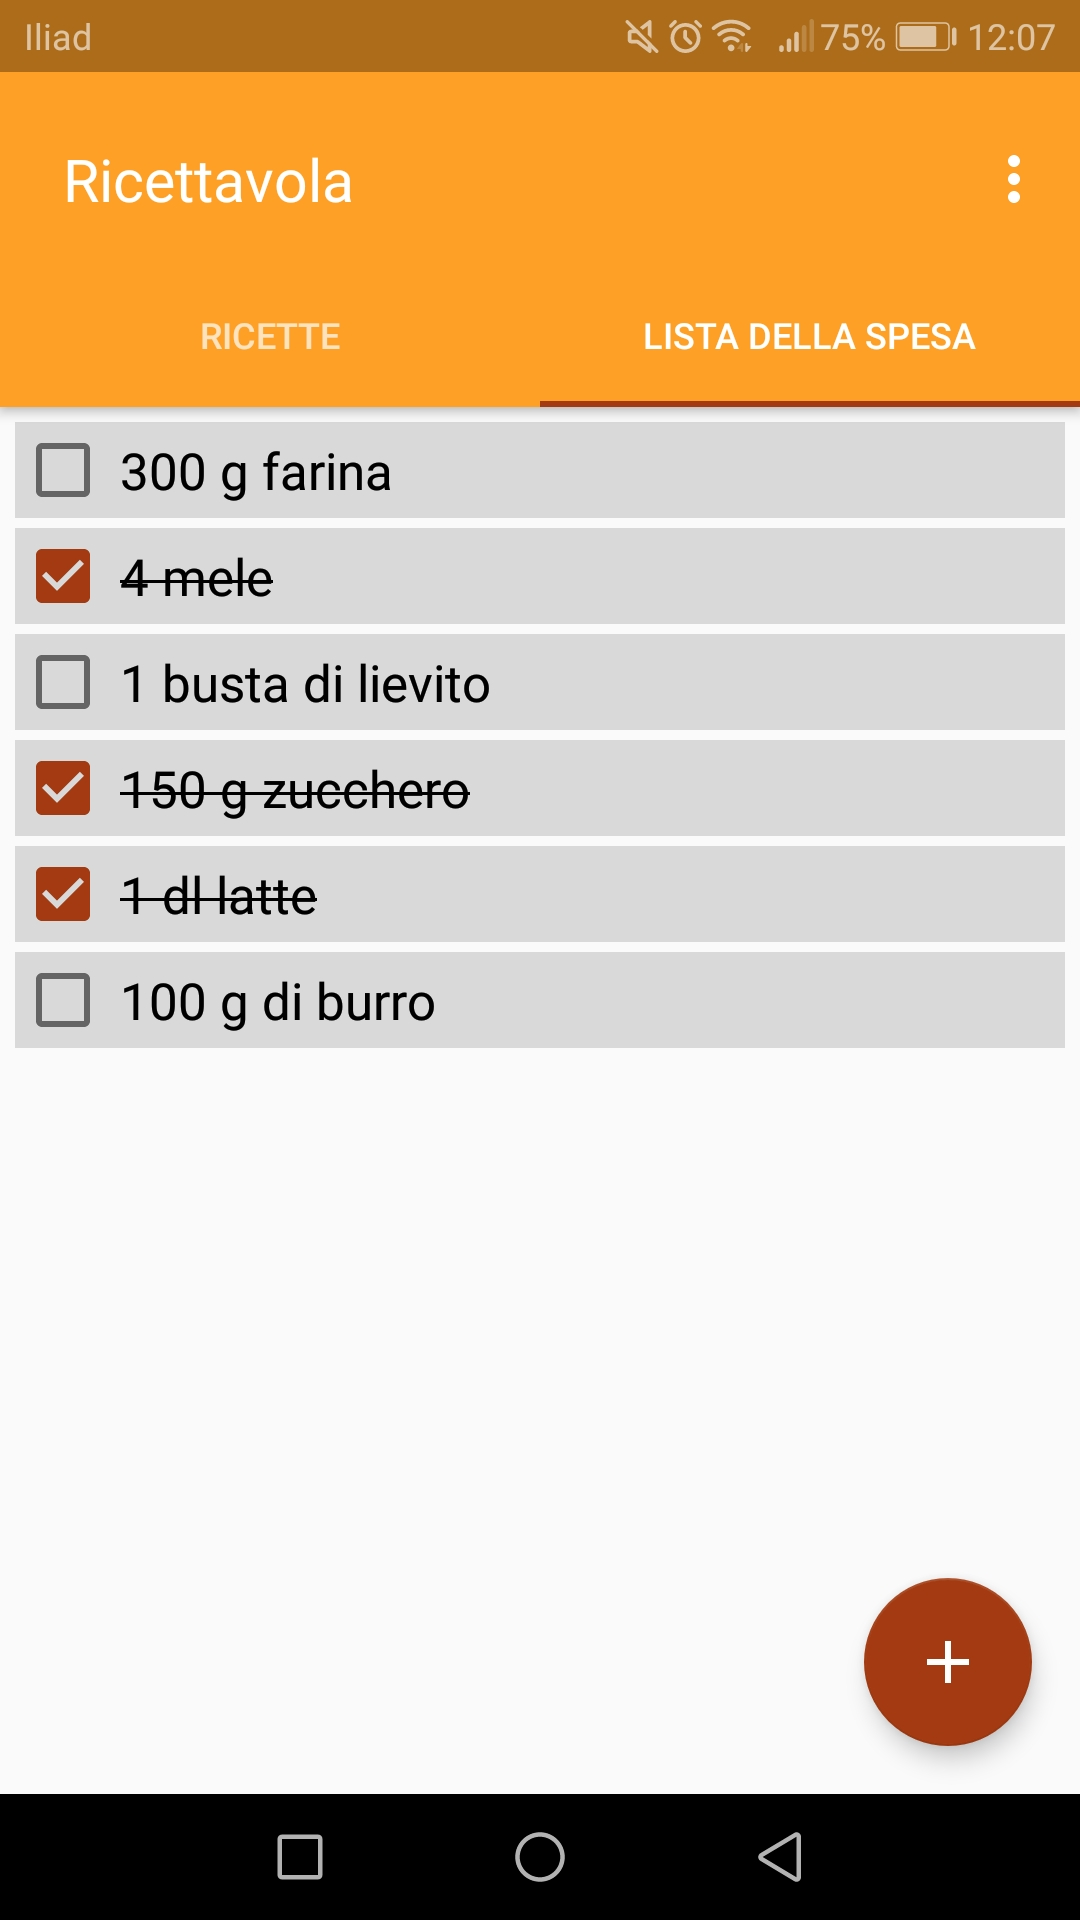
\includegraphics[width=0.49\textwidth]{definitivo/lista_della_spesa}
    \caption{Schermata principale}
    \label{fig:def_main}
  \end{center}
\end{figure}

Tendo premuto su una ricetta è possibile far comparire un cestino per ogni elemento.
Se l'icona viene premuta compare una messaggio come quello in figura \ref{fig:def_main_3}.
Notare che le due immagini corrispondono allo stesso messaggio, ma nel secondo la lingua dell'applicazione è impostata sull'inglese.

\begin{figure}[ht]
  \begin{center}
    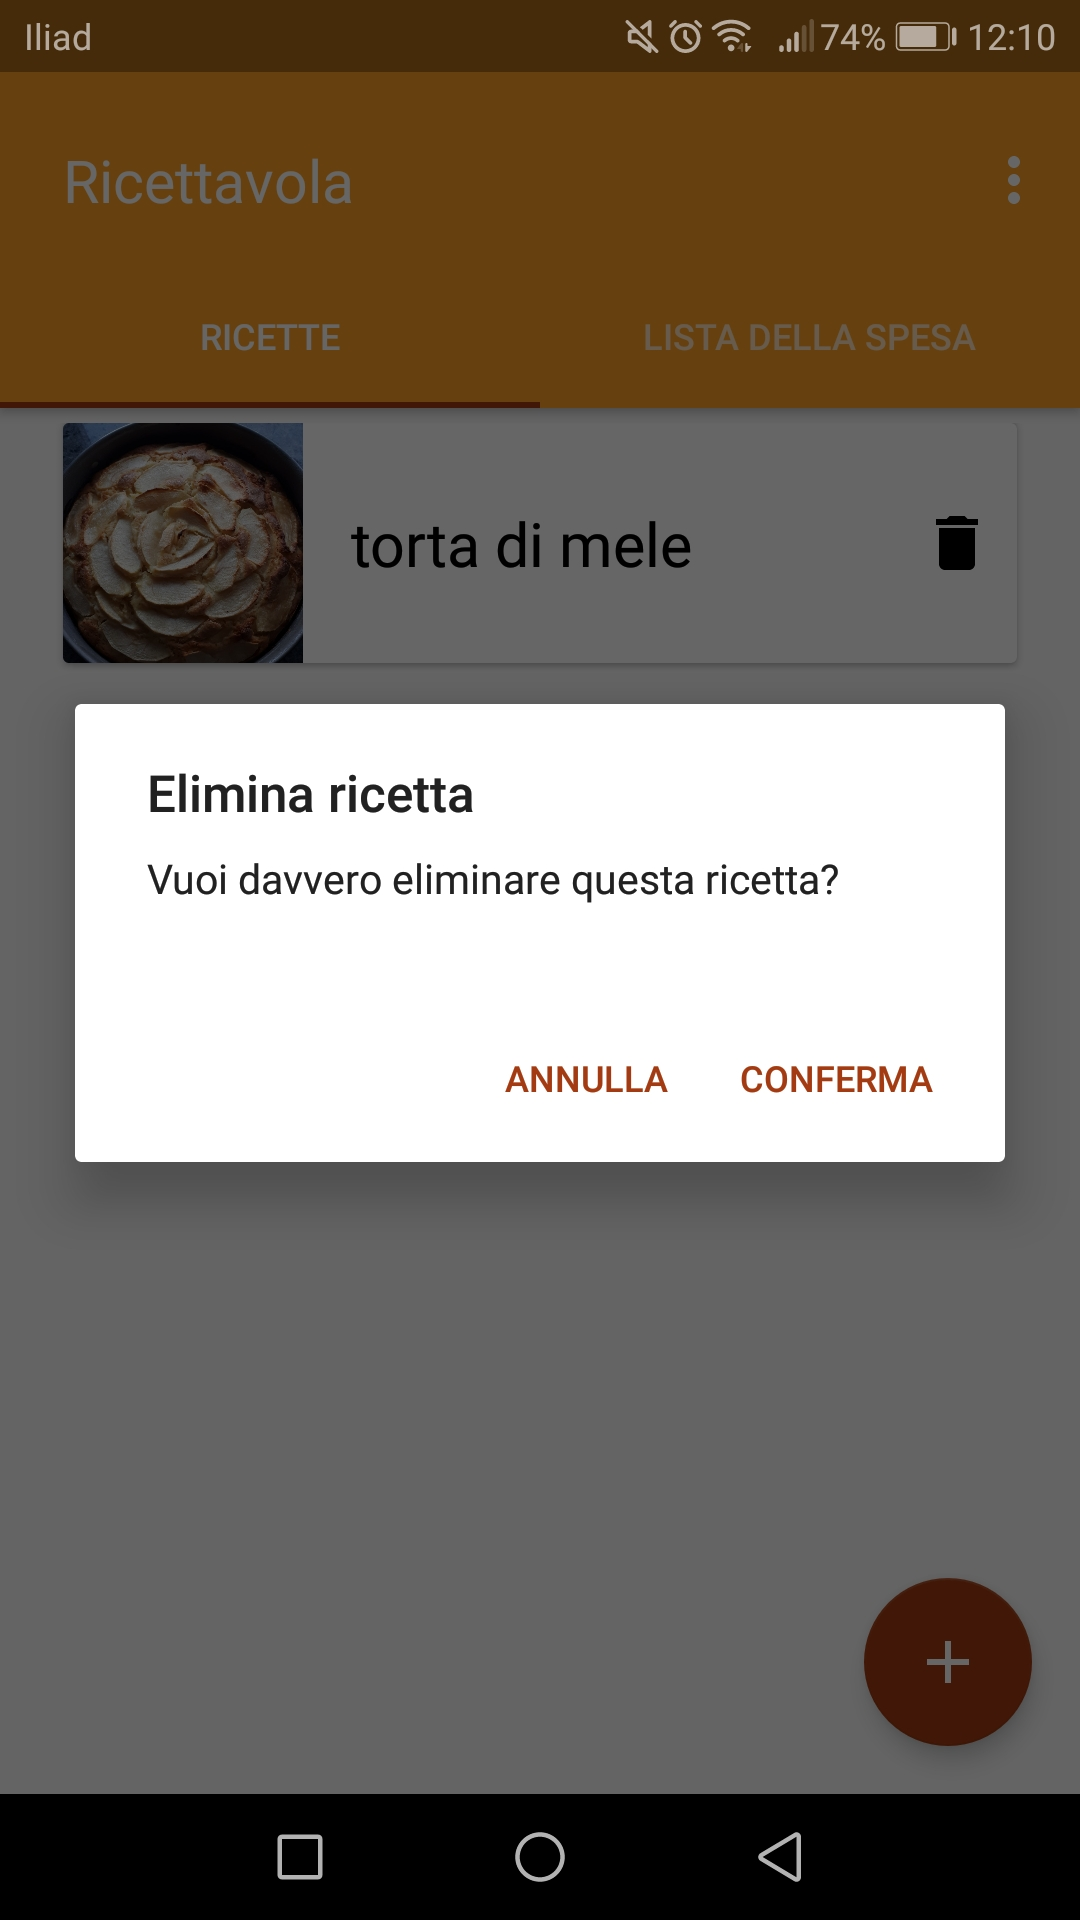
\includegraphics[width=0.49\textwidth]{definitivo/elimina_ricetta}
    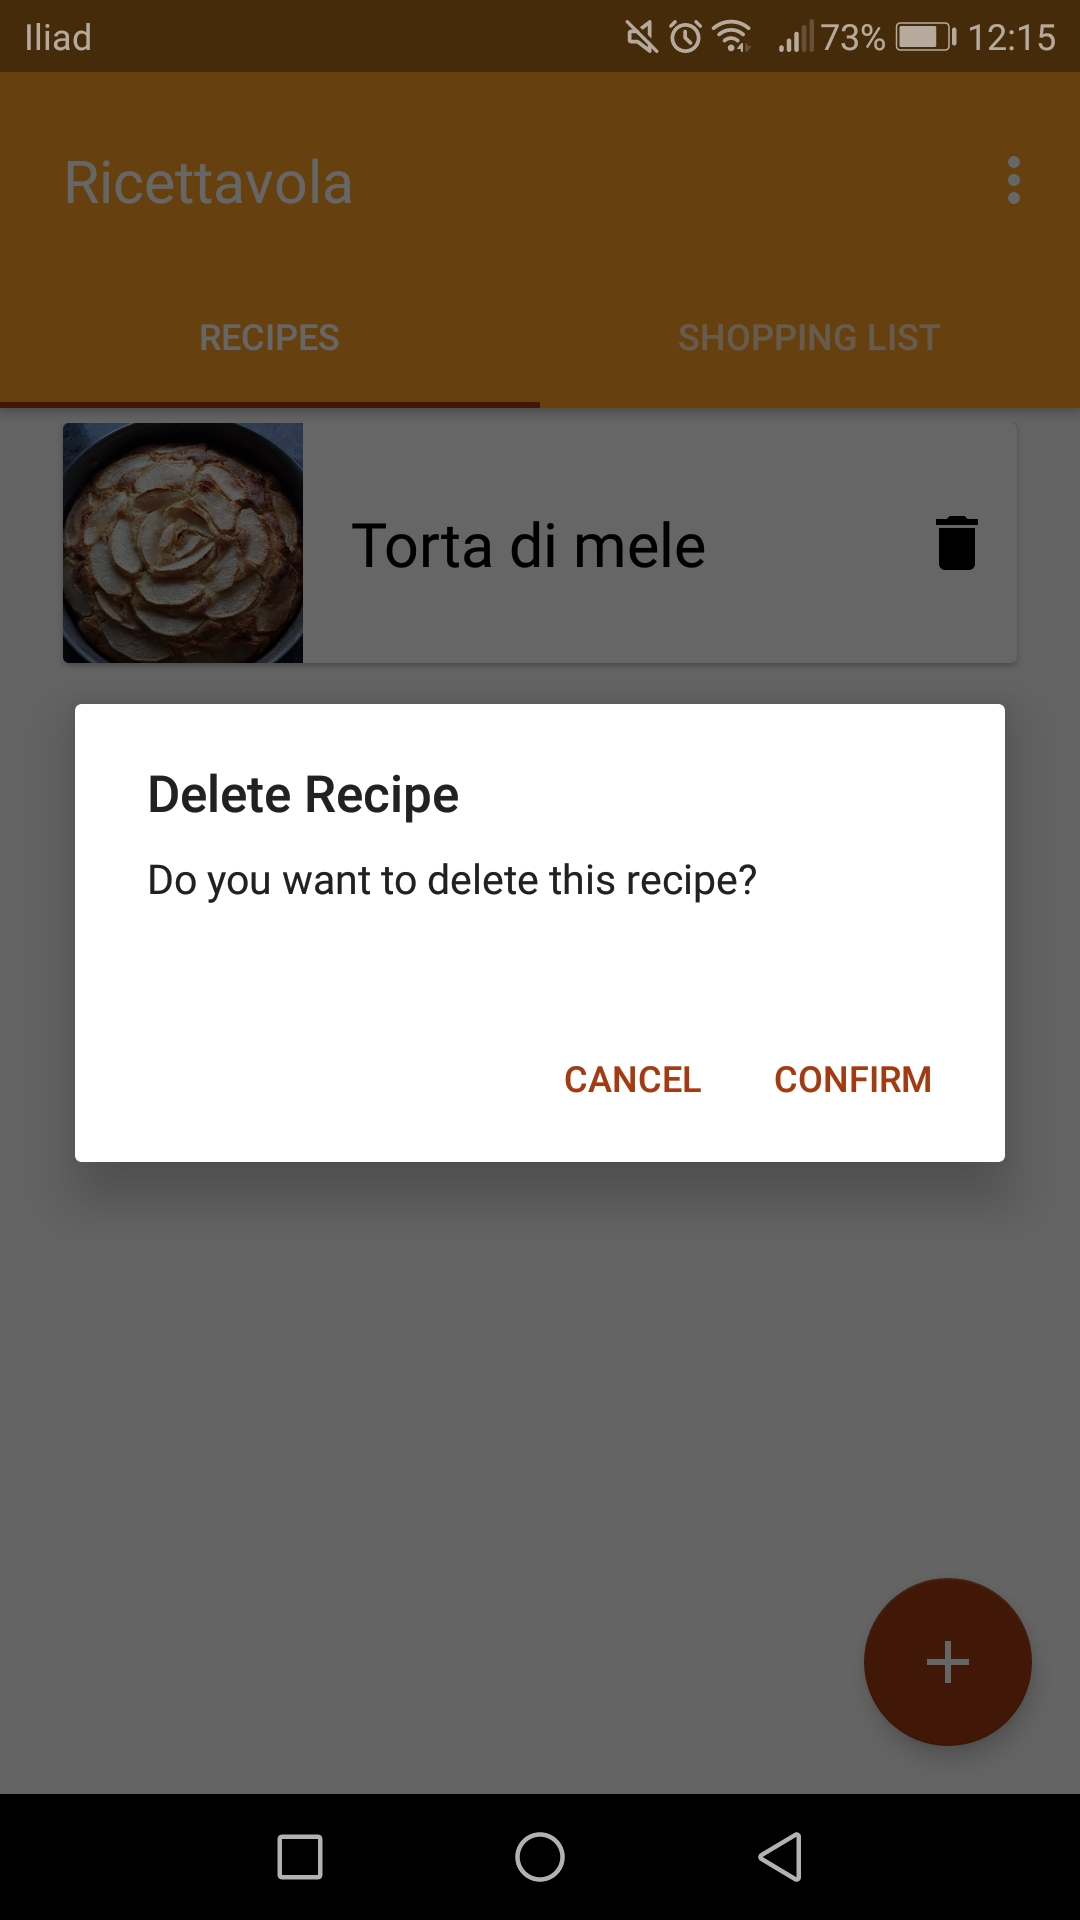
\includegraphics[width=0.49\textwidth]{definitivo/elimina_ricetta_eng}
    \caption{Messaggio di conferma eliminazione ricetta}
    \label{fig:def_main_3}
  \end{center}
\end{figure}

In figura \ref{fig:def_main_2} è illustrato il menù a tendina dell'attività principale.
L'ultima voce, a prescindere dalla lingua, riporta "Change language" così la sua funzione rimane chiara indipendentemente dalla lingua attuale.
Premendo questa voce si può ruotare tra due lingue: italiano ed inglese.
Appena sopra sono presenti due voci per la manipolazione della lista della spesa.
Premendo "Aggiungi ricetta da clipboard" verrà verificato se il testo nella \textit{clipboard} corrisponde a quello di una ricetta.
In caso affermativo la ricetta apparirà nell'elenco delle ricette, altrimenti comparirà un messaggio d'errore.

\begin{figure}[ht]
  \begin{center}
    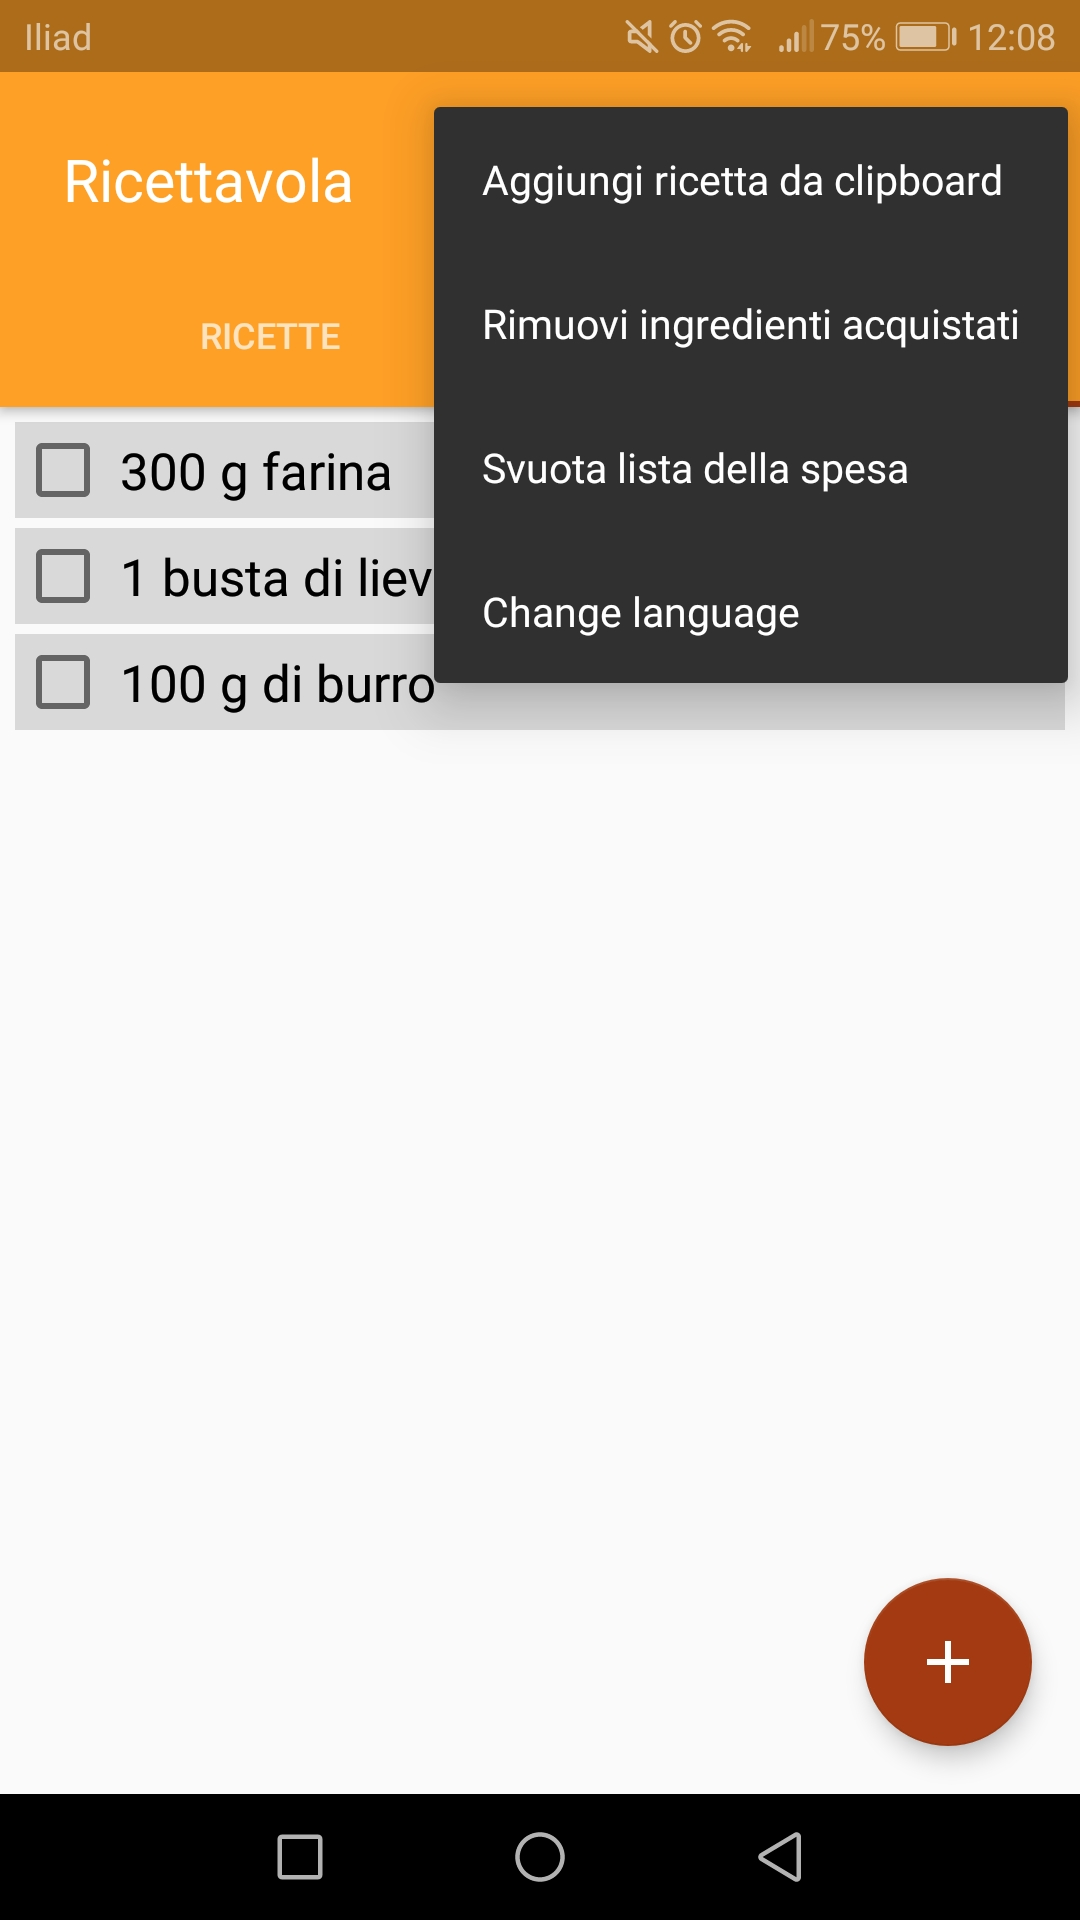
\includegraphics[width=0.8\textwidth]{definitivo/menu_main}
    \caption{Menù schermata principale}
    \label{fig:def_main_2}
  \end{center}
\end{figure}
\clearpage

Premendo il tasto per aggiungere una ricetta verrà mostrata la schermata in figura \ref{fig:def_nuova}.
\begin{figure}[ht]
  \begin{center}
    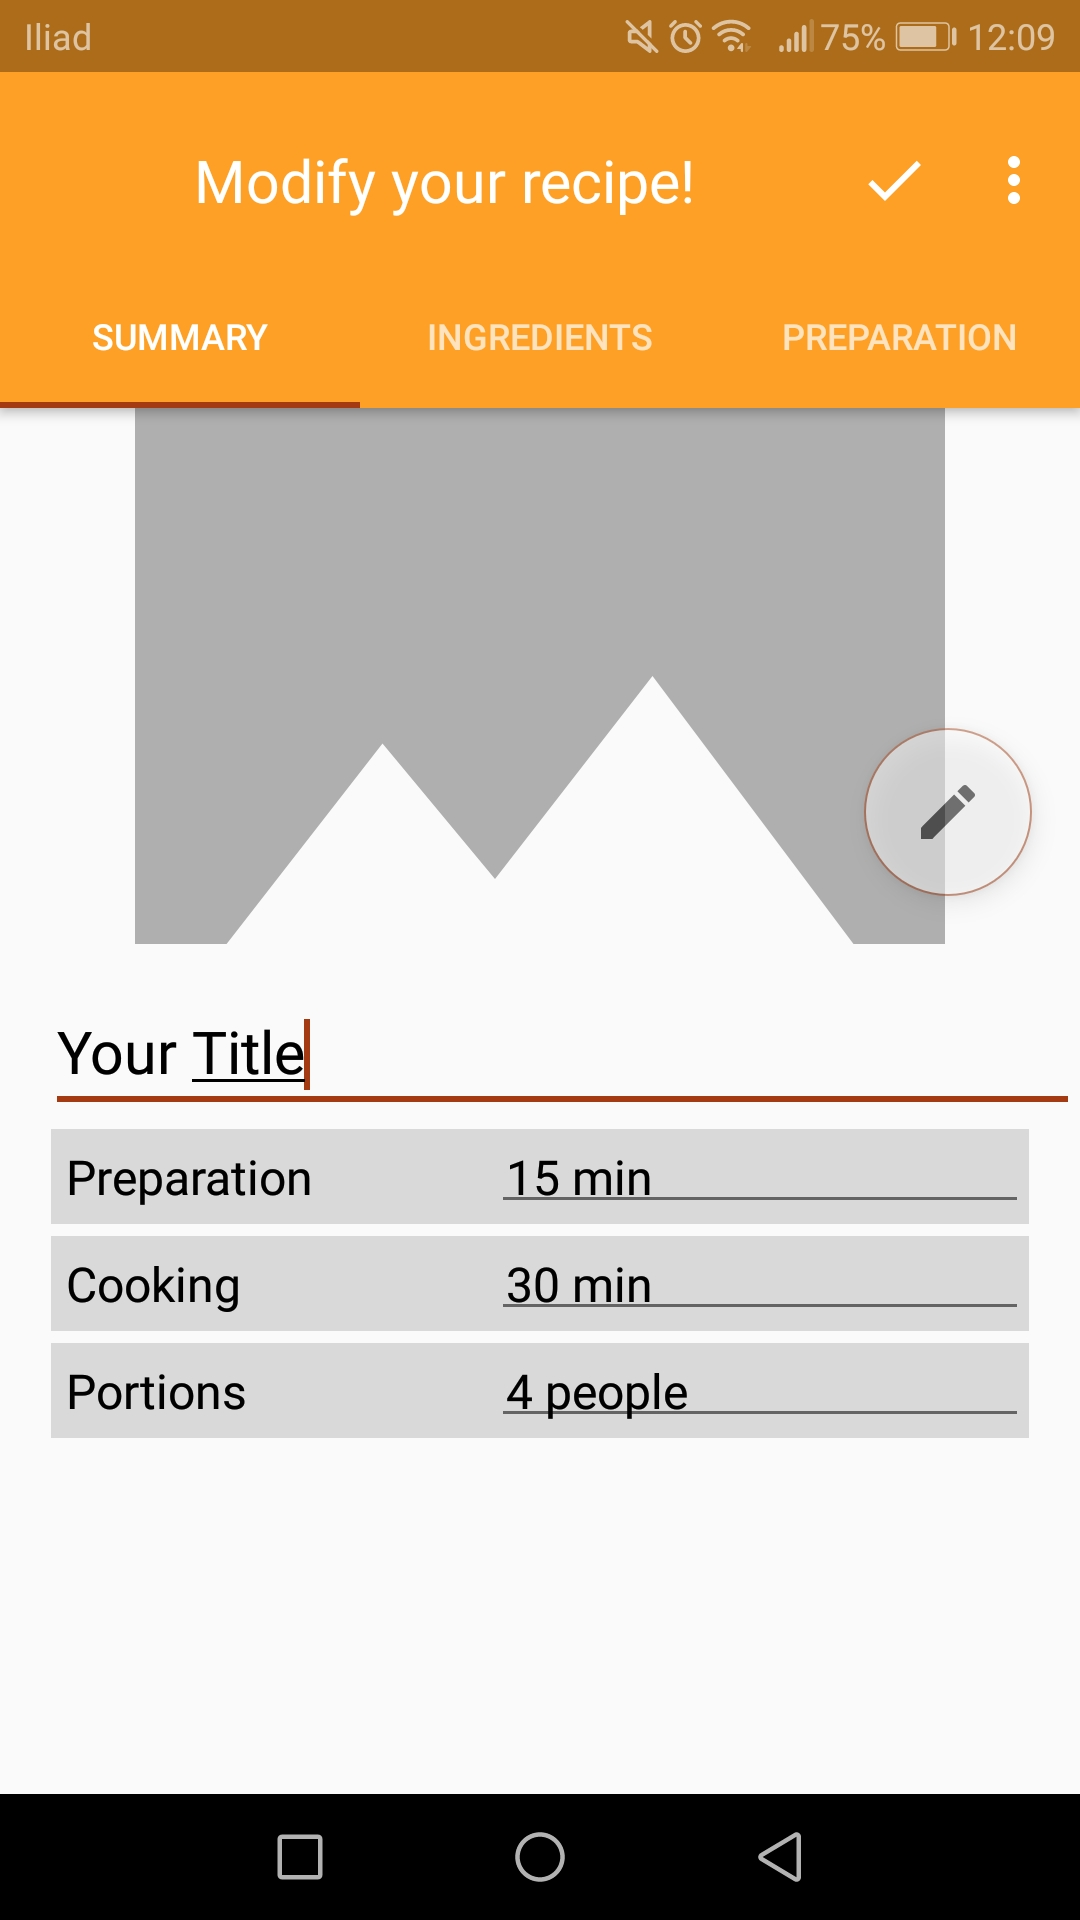
\includegraphics[width=0.6\textwidth]{definitivo/nuova_ricetta_eng}
    \caption{Schermata di una nuova ricetta}
    \label{fig:def_nuova}
  \end{center}
\end{figure}

\begin{figure}[ht]
  \begin{center}
    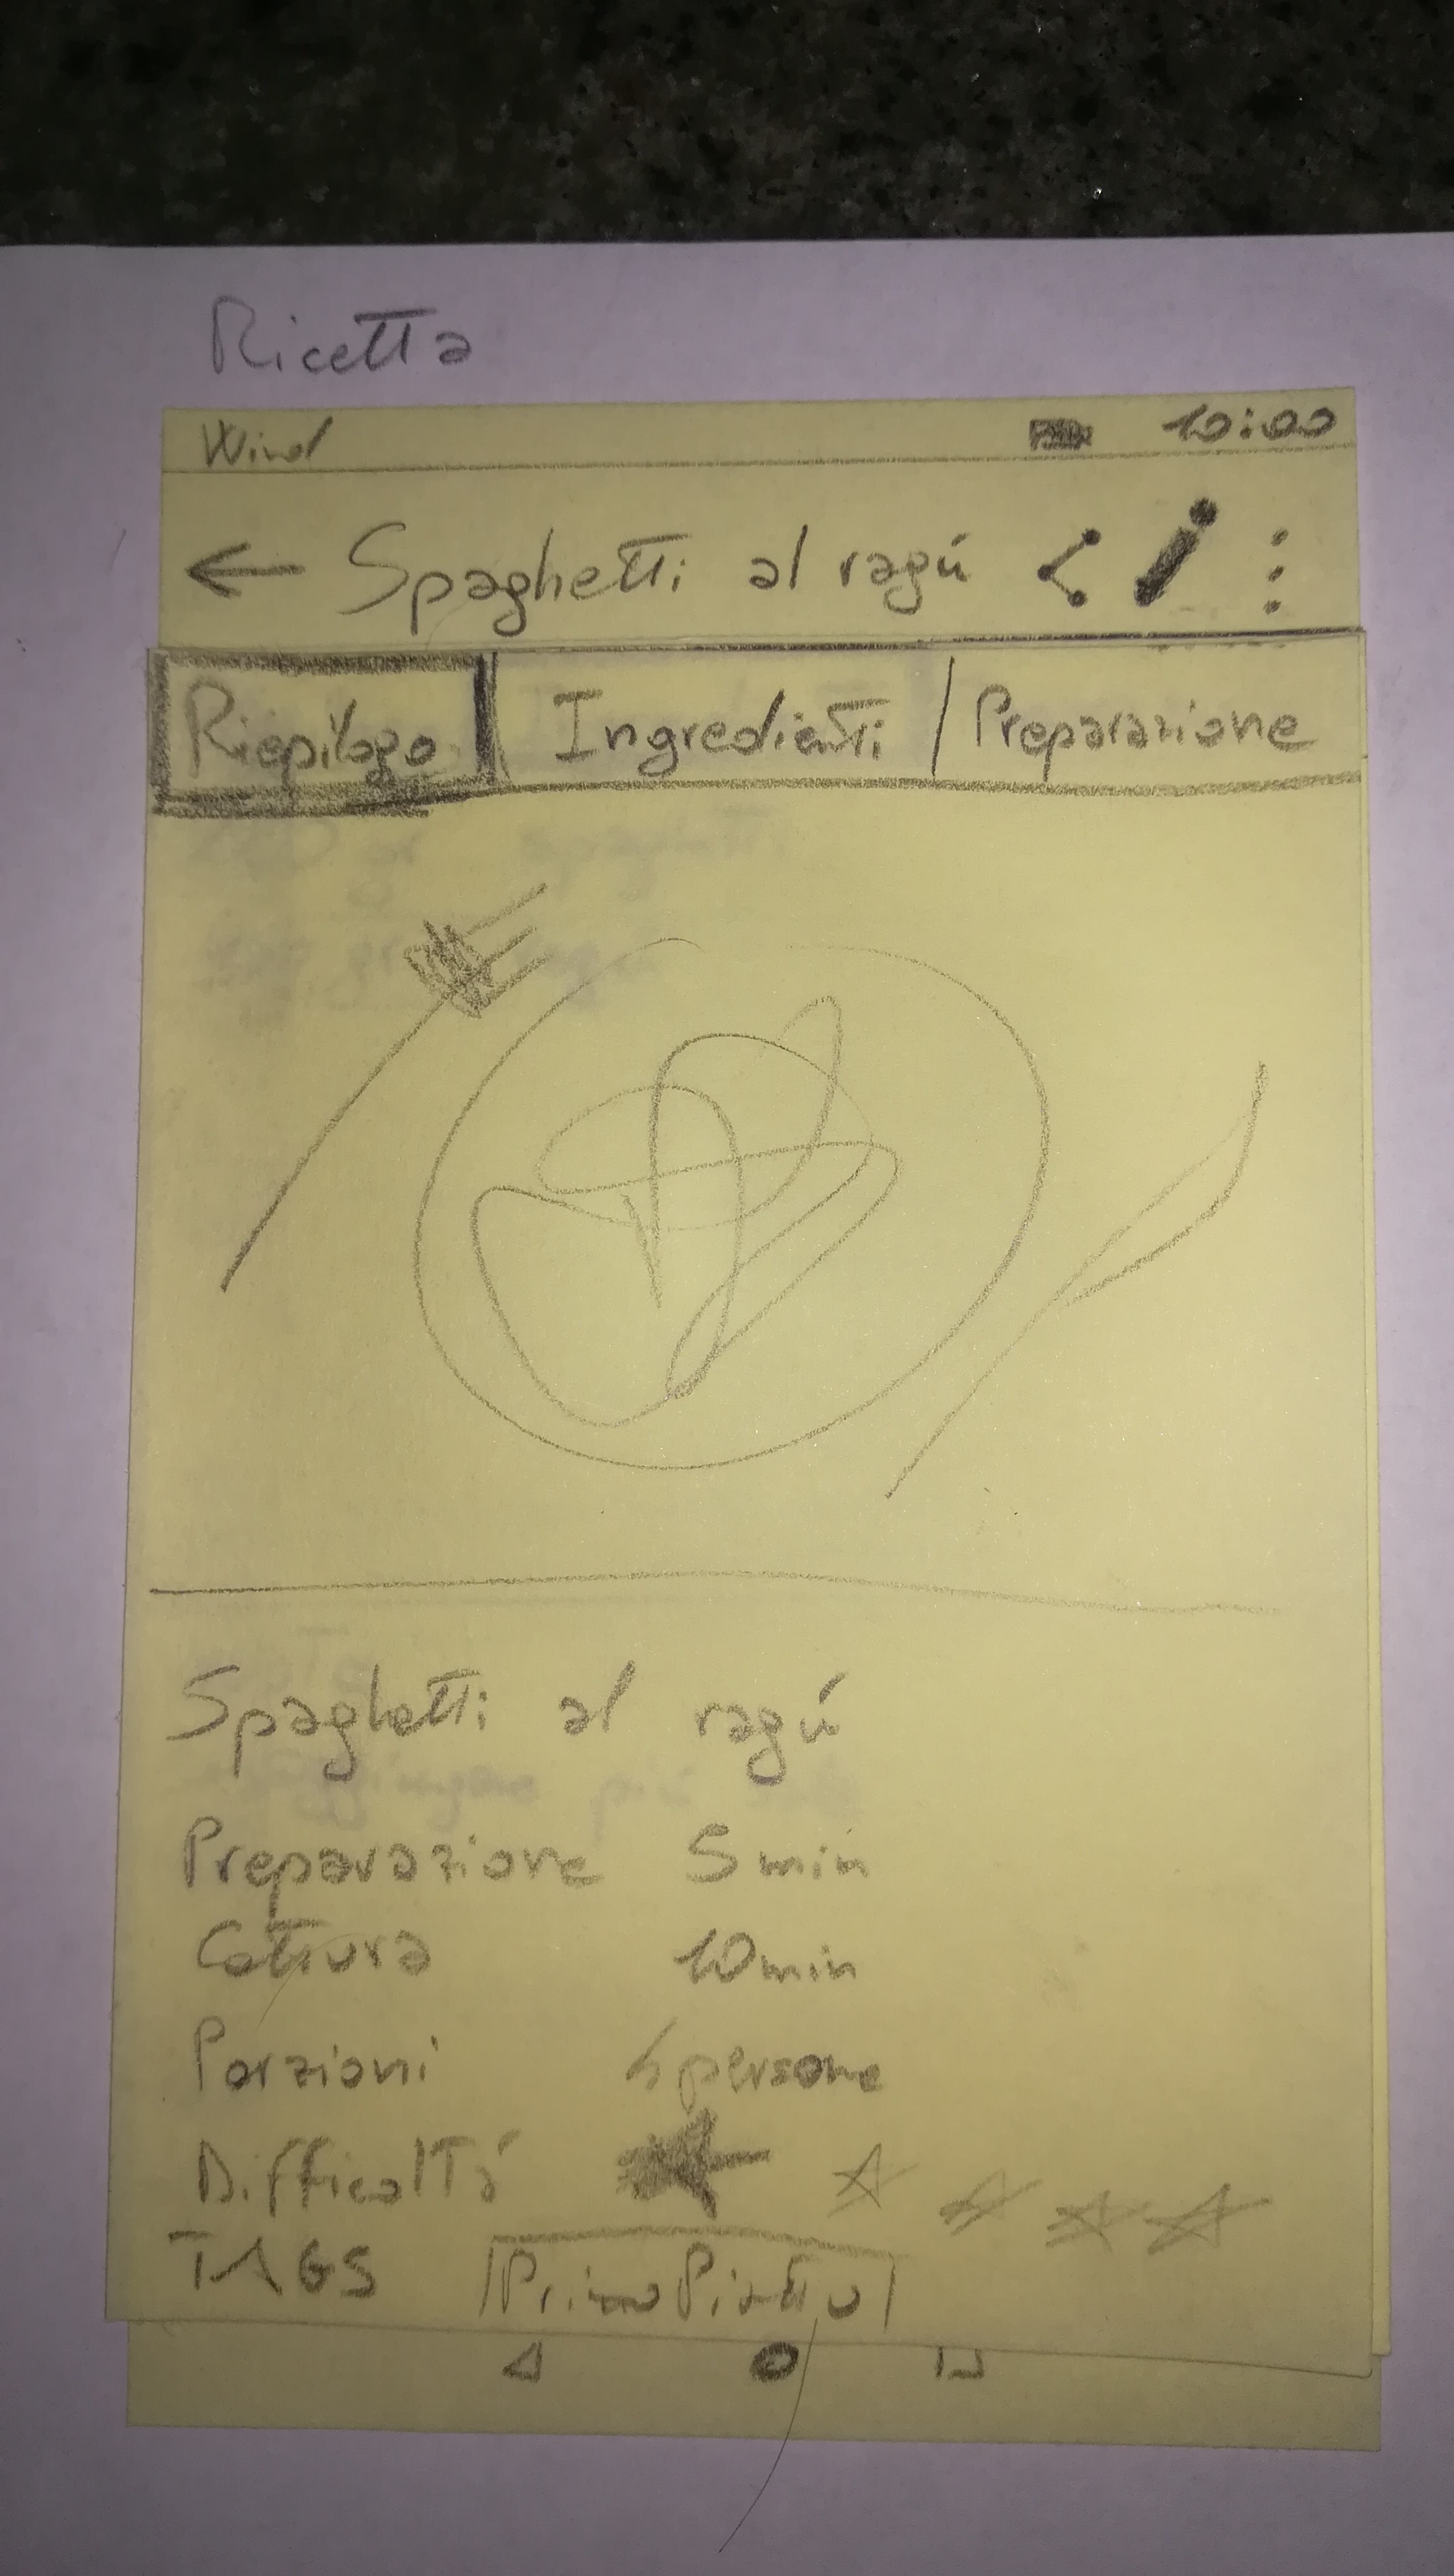
\includegraphics[width=0.49\textwidth]{definitivo/ricetta_riepilogo}
    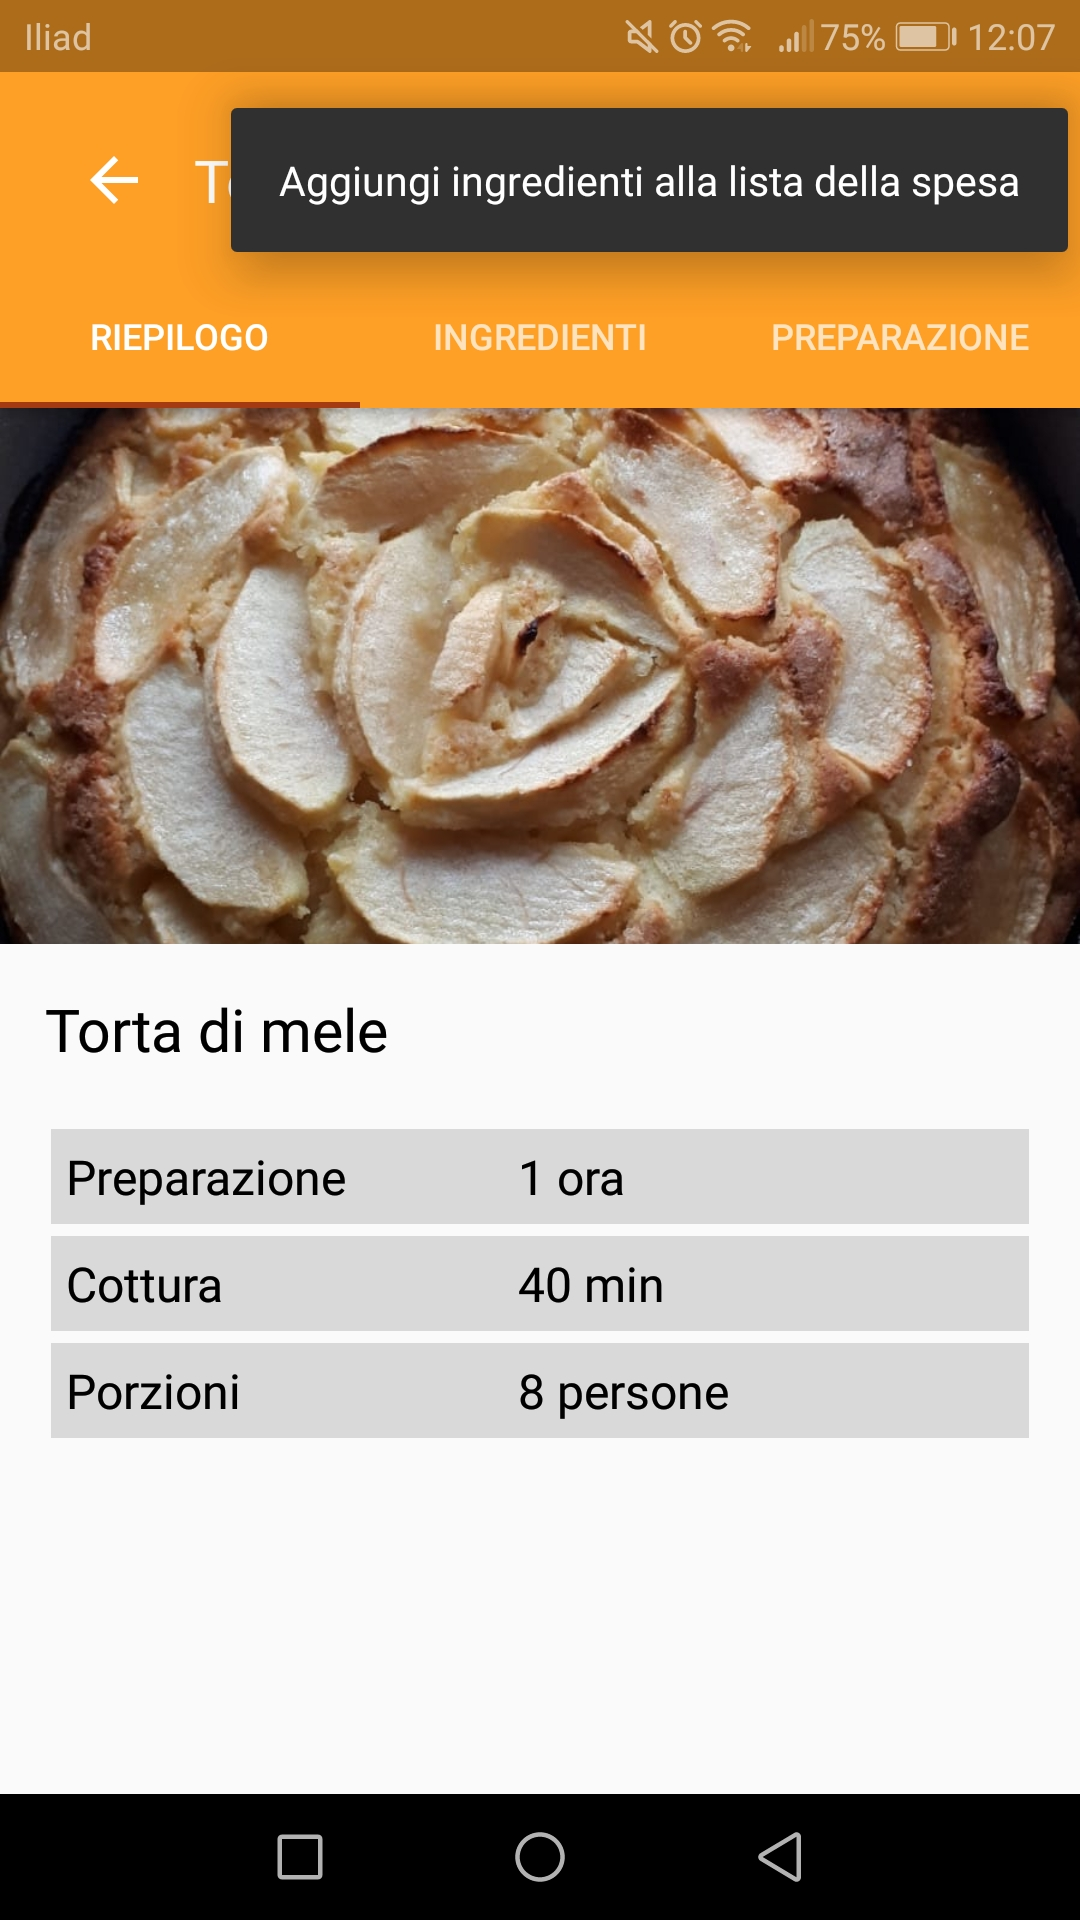
\includegraphics[width=0.49\textwidth]{definitivo/menu_riepilogo}
    \caption{Schermata di riepilogo di una ricetta e suo menù}
    \label{fig:def_ricetta}
  \end{center}
\end{figure}

\begin{figure}[ht]
  \begin{center}
    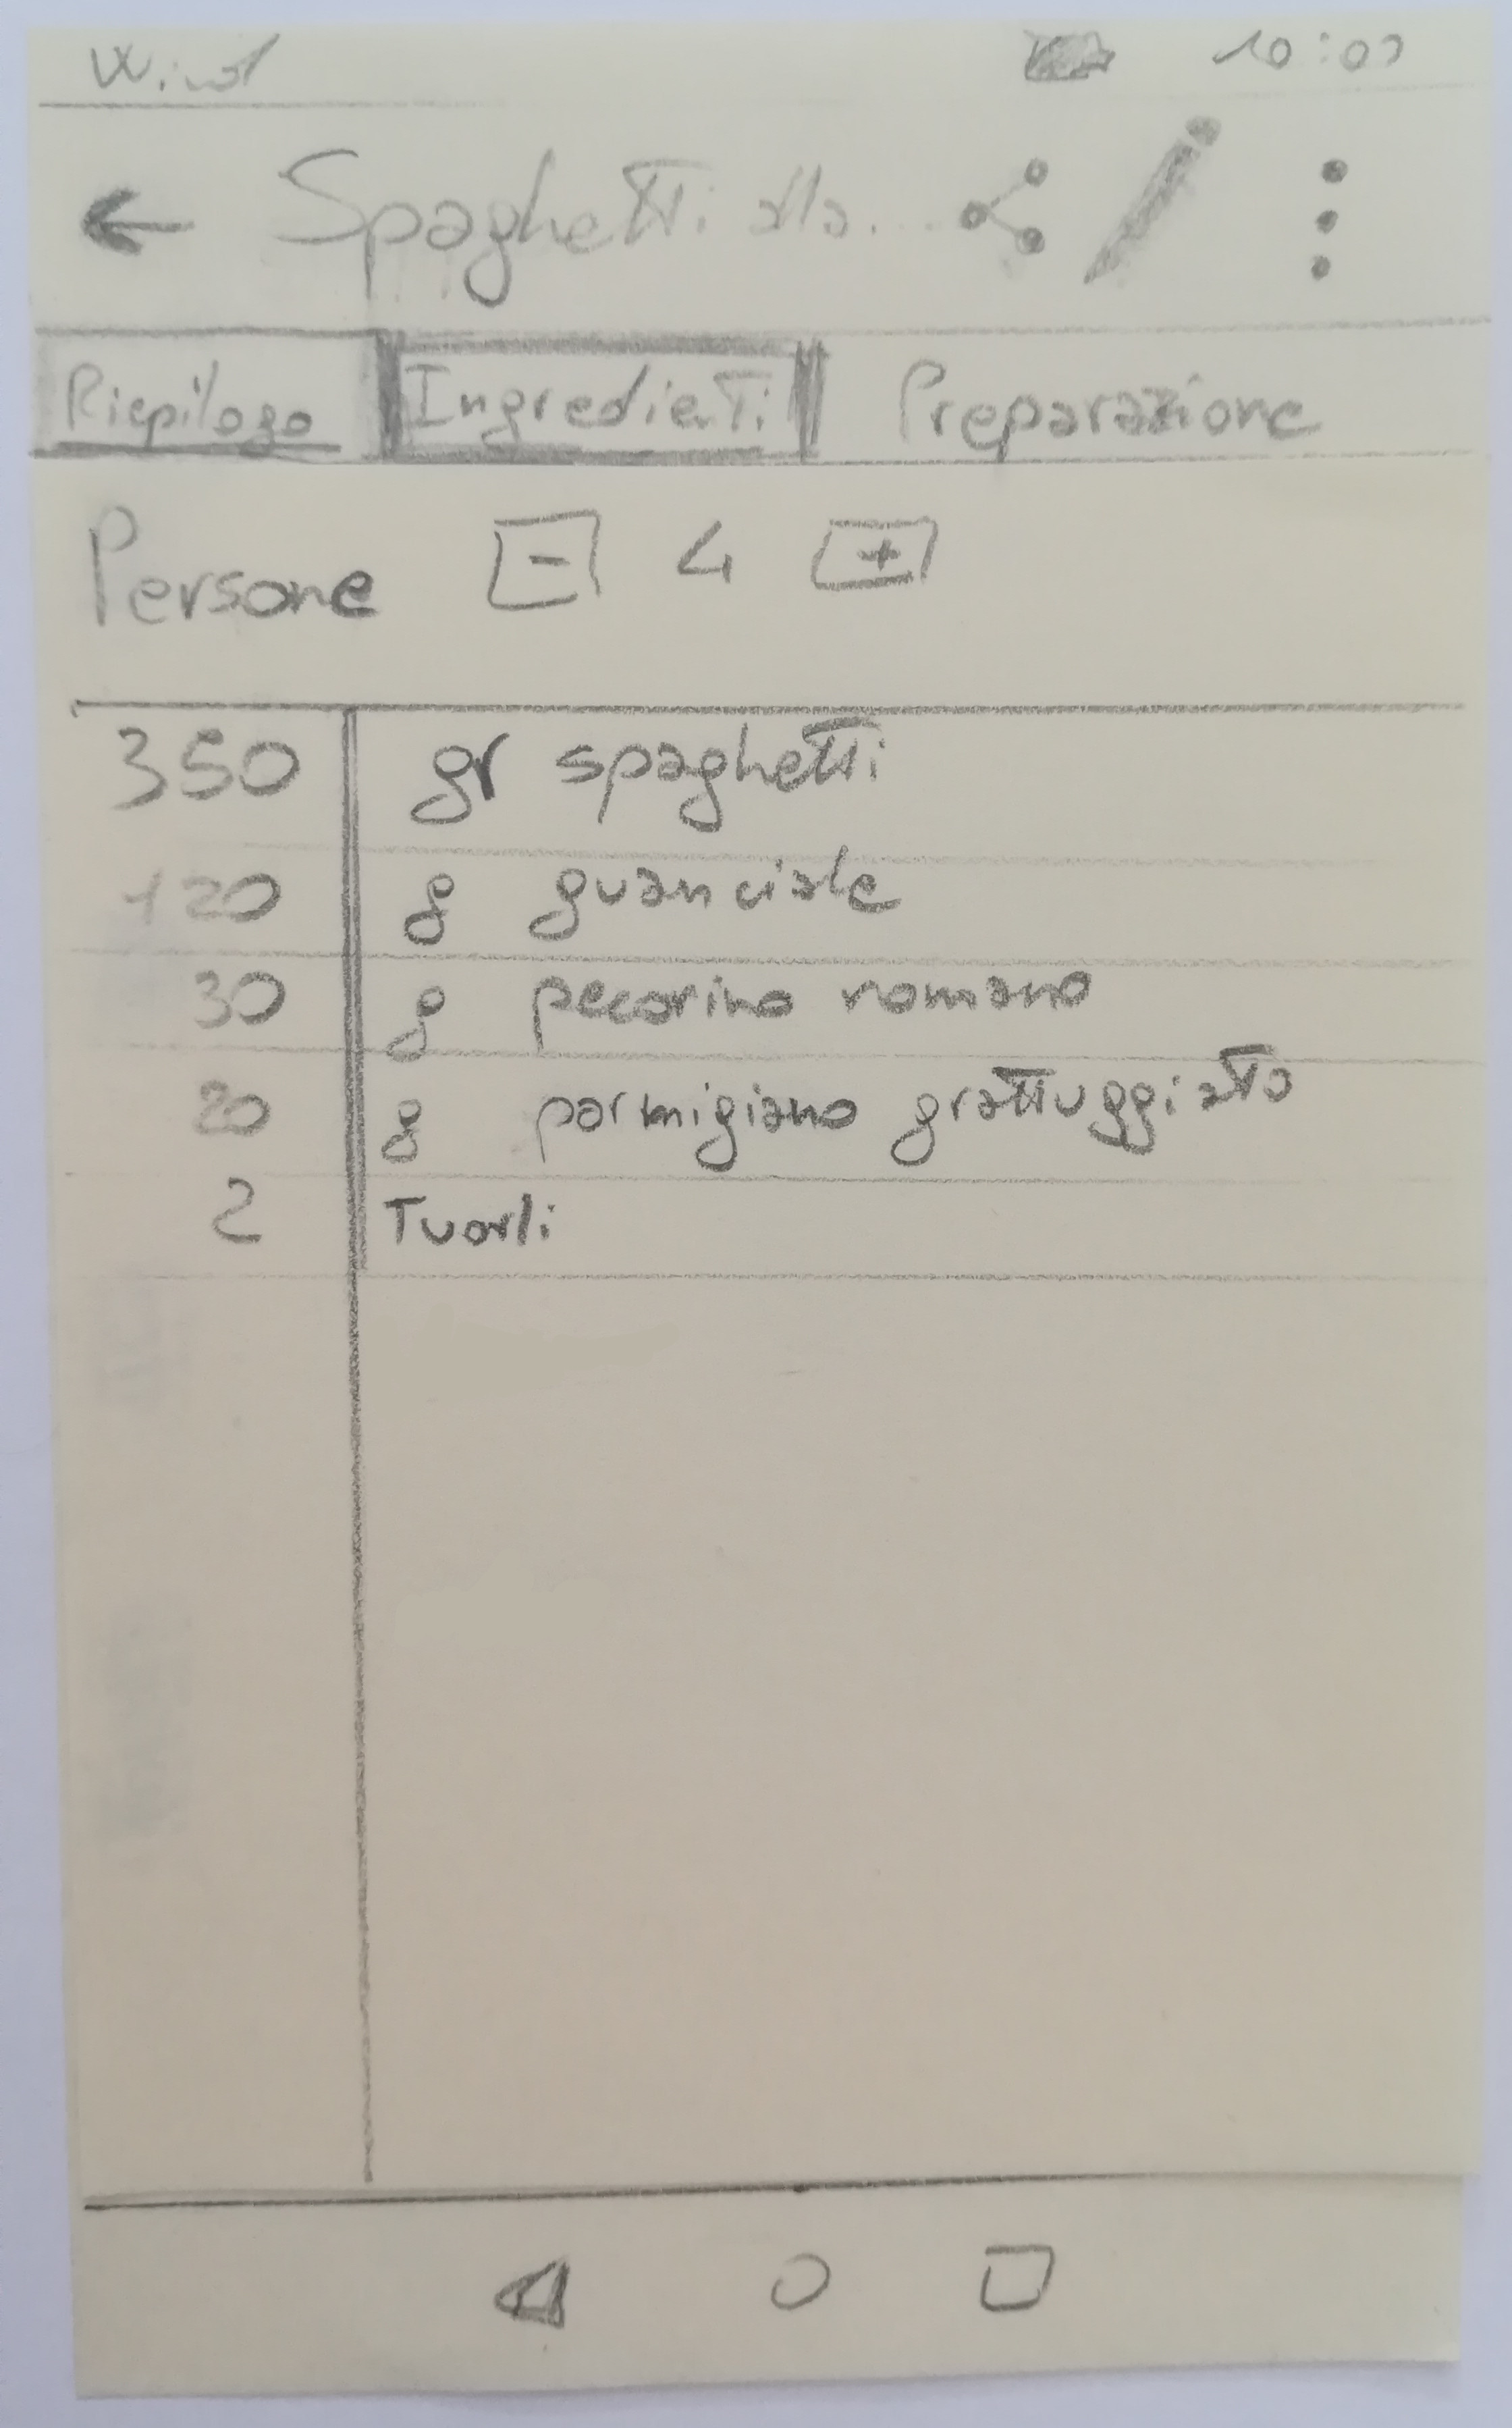
\includegraphics[width=0.49\textwidth]{definitivo/ricetta_ingredienti}
    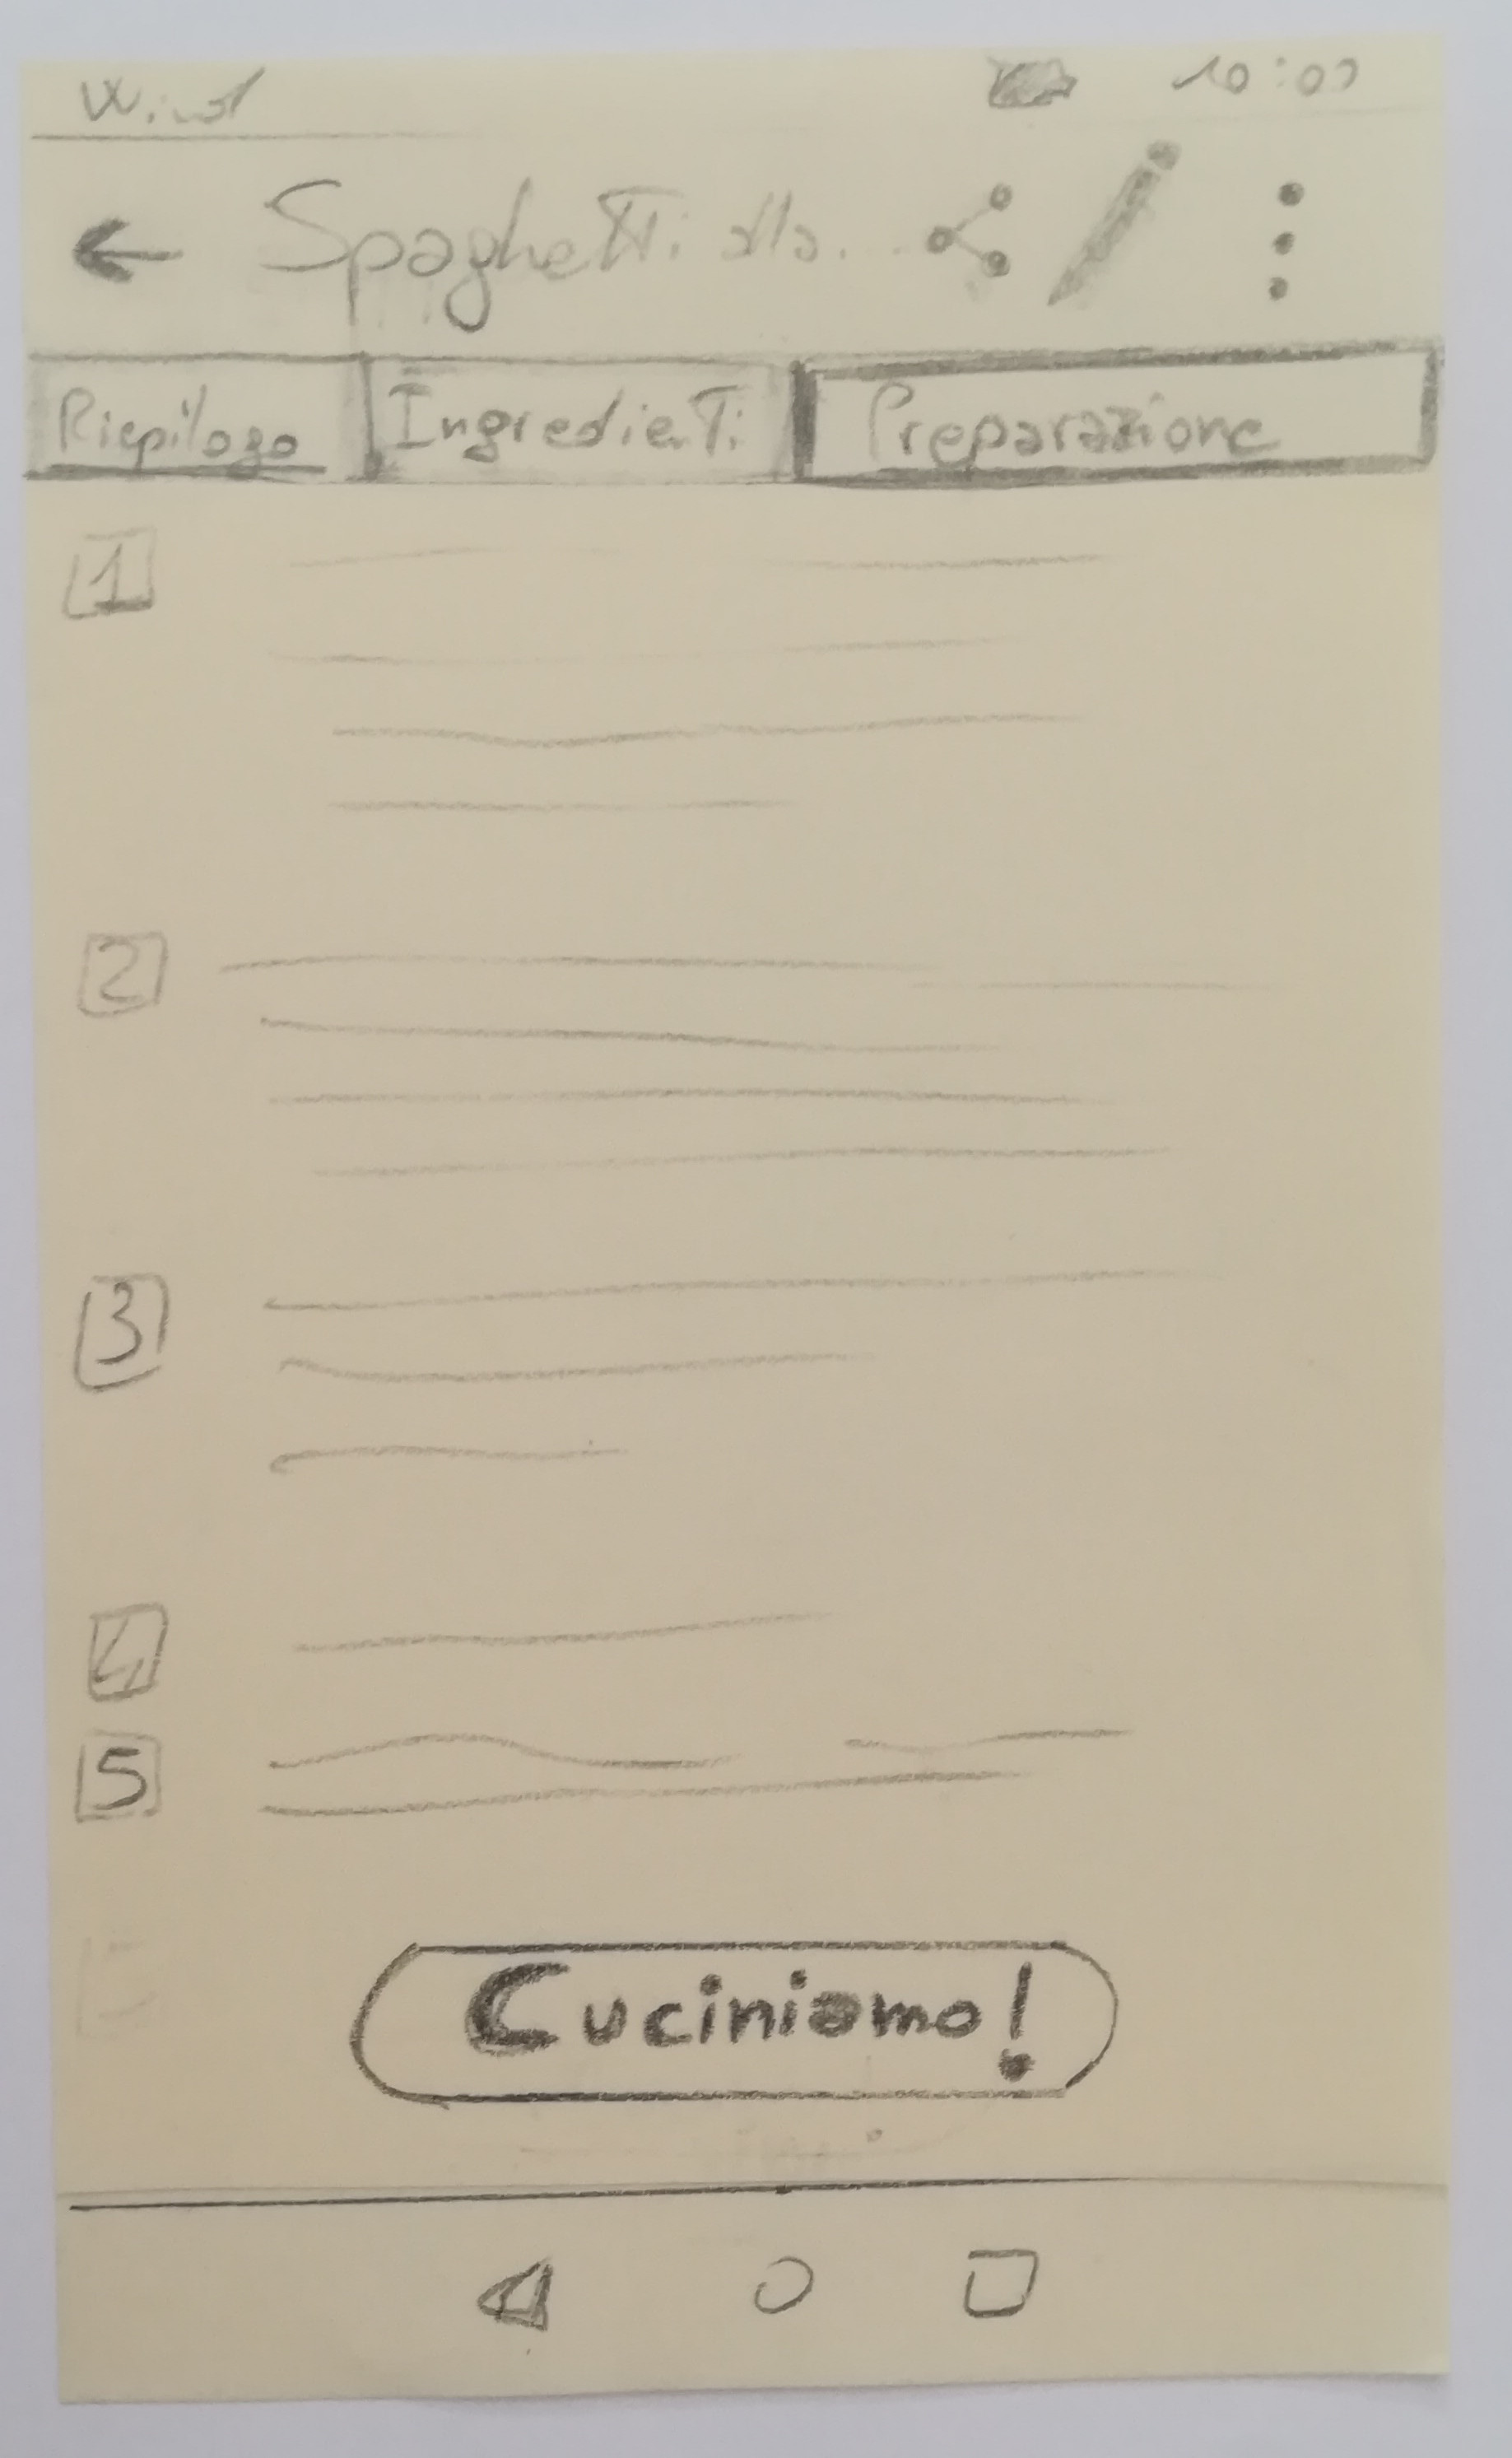
\includegraphics[width=0.49\textwidth]{definitivo/ricetta_preparazione}
    \caption{Schermate ingredienti e preparazione}
    \label{fig:def_ricetta_1}
  \end{center}
\end{figure}

\begin{figure}[ht]
   \begin{center}
    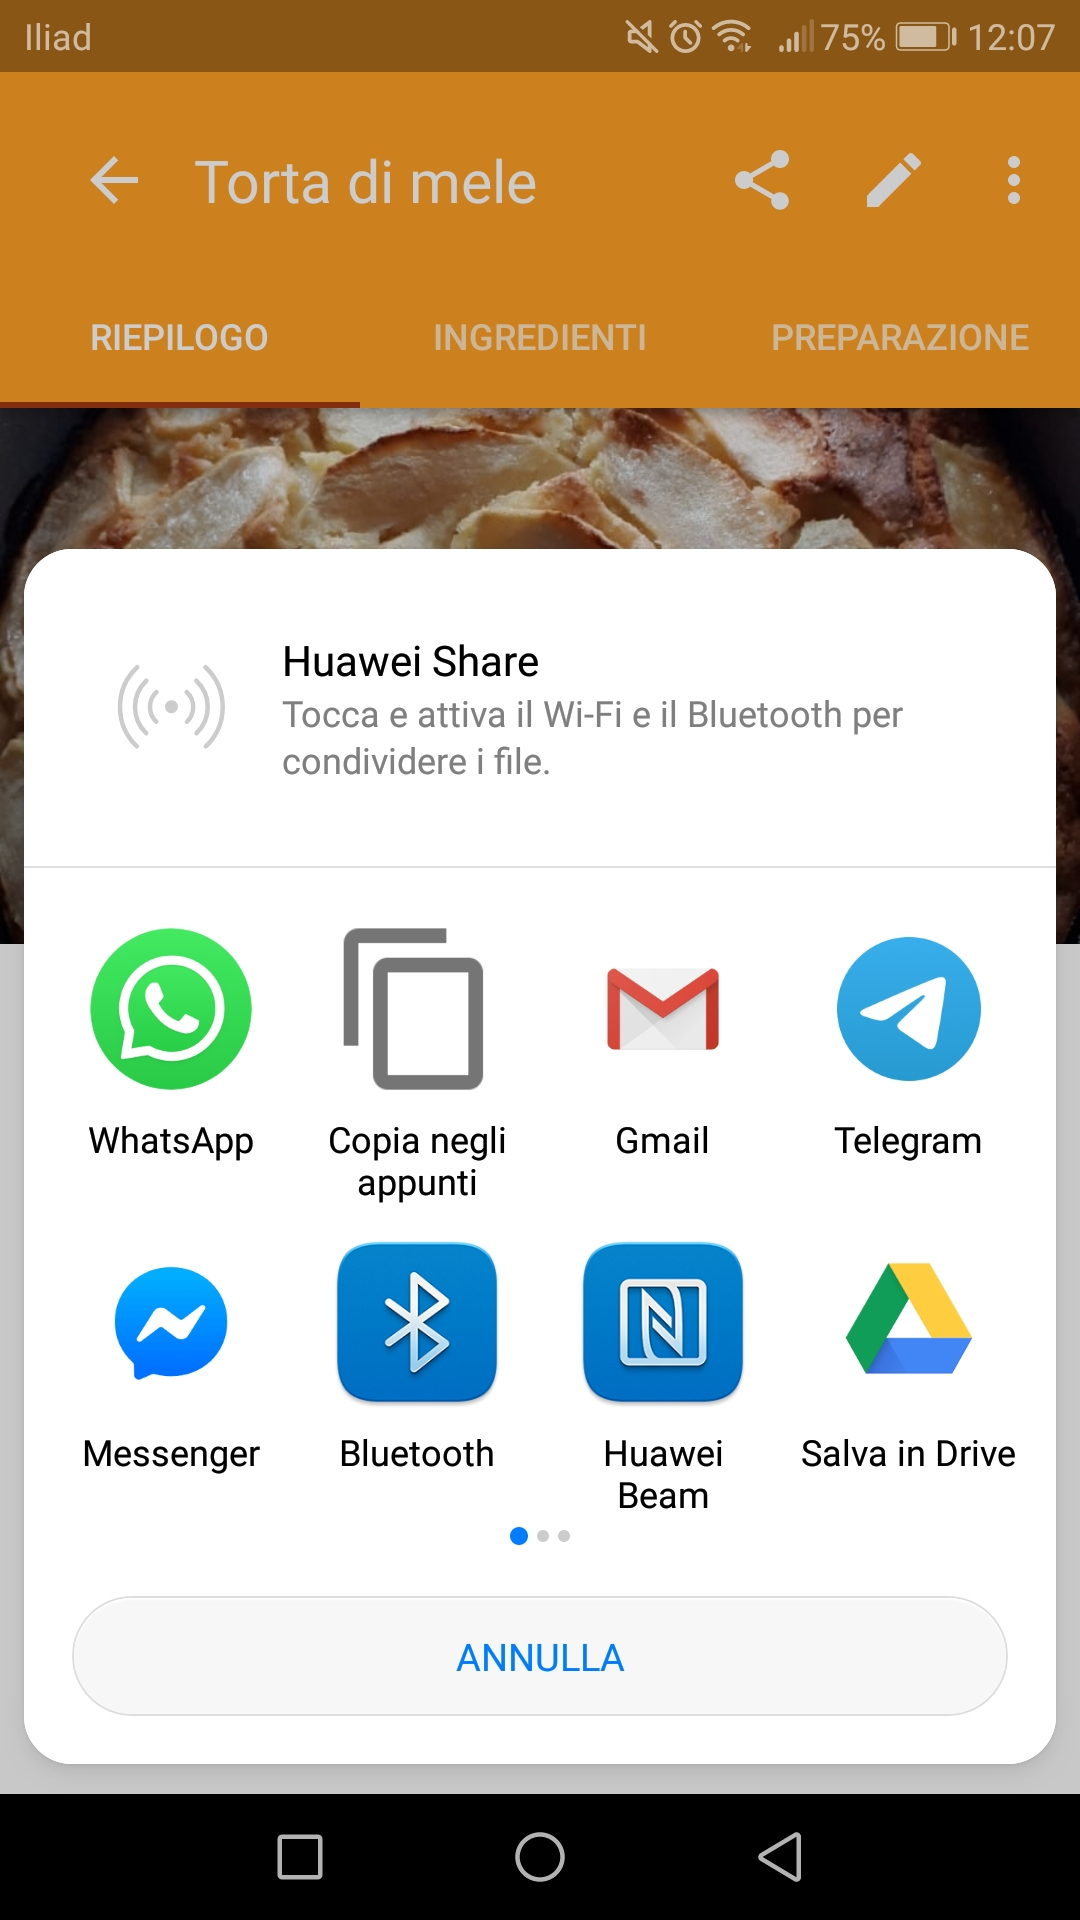
\includegraphics[width=0.49\textwidth]{definitivo/tasto_share}
    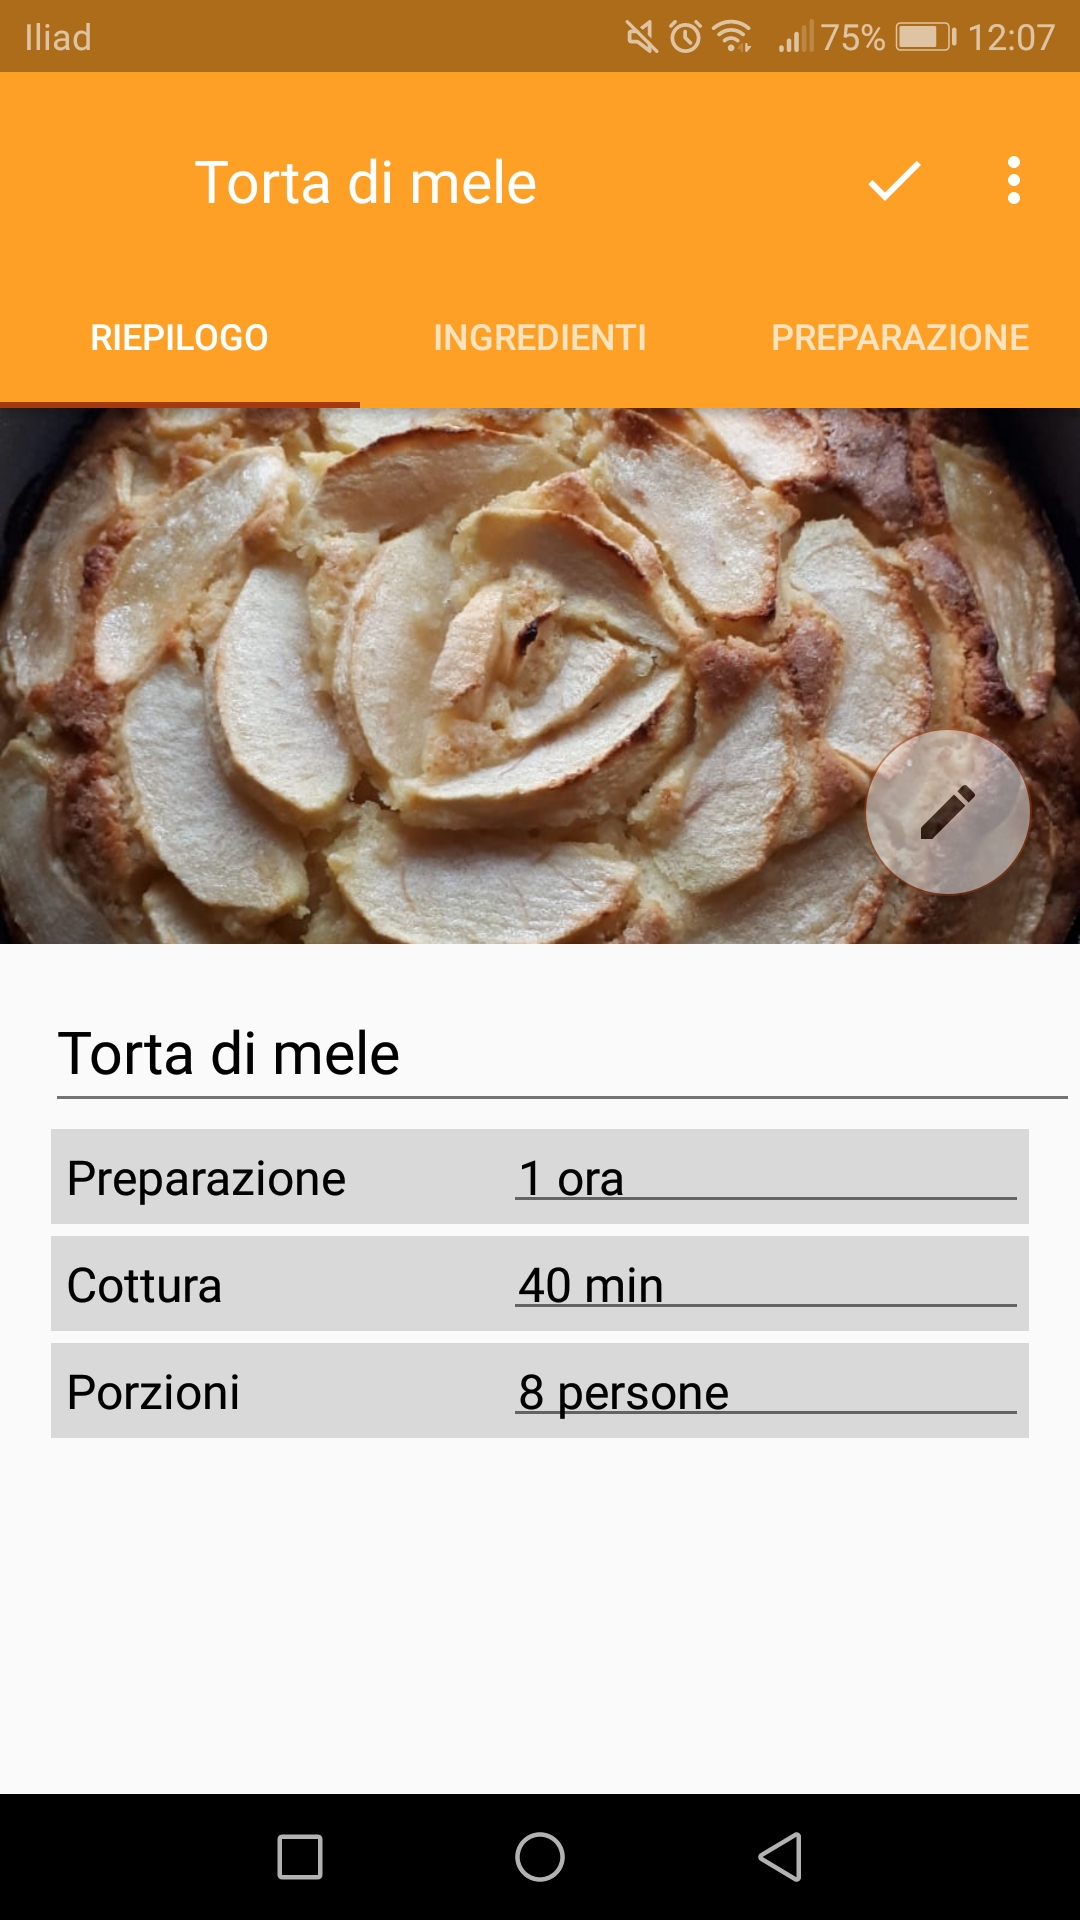
\includegraphics[width=0.49\textwidth]{definitivo/edit_riepilogo}
    \caption{Azione di condivisione e modifica del riepilogo}
    \label{fig:def_ricetta_2}
  \end{center}
\end{figure}

\begin{figure}[ht]
  \begin{center}
    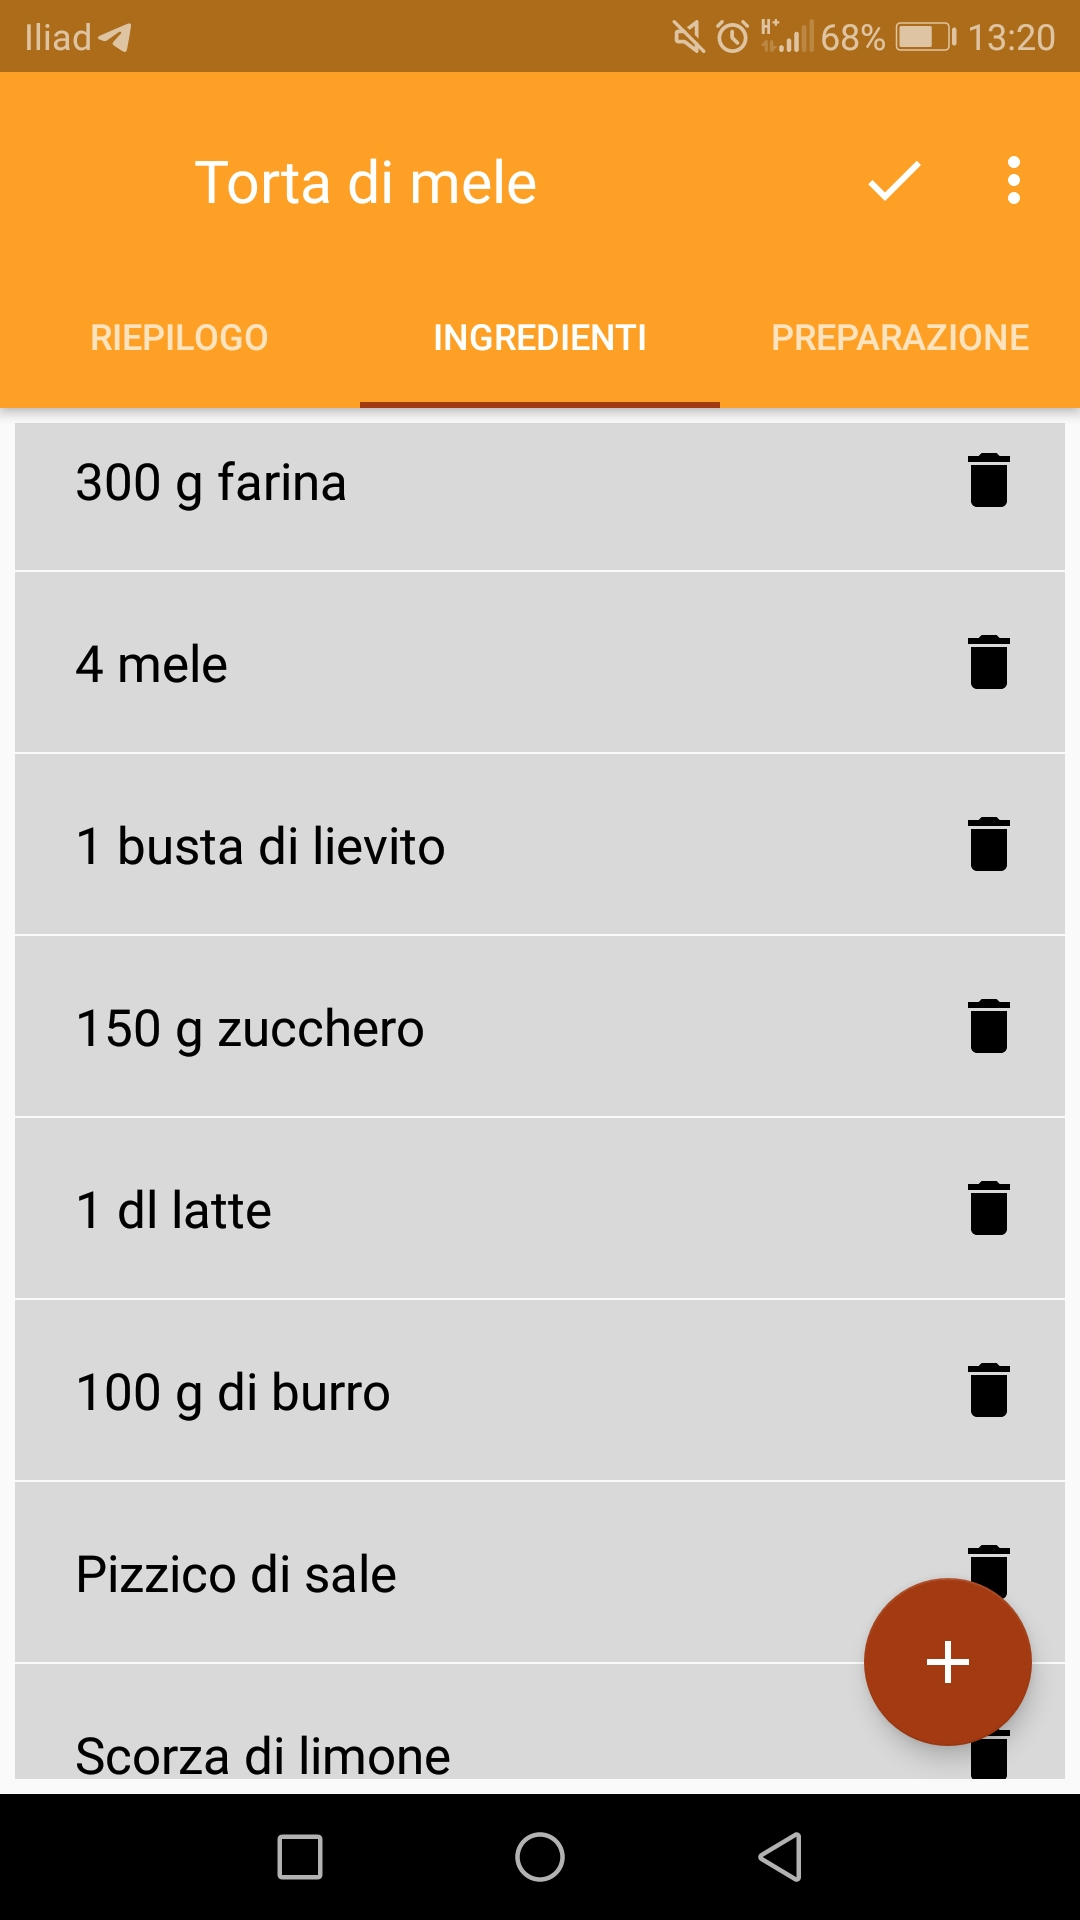
\includegraphics[width=0.49\textwidth]{definitivo/edit_ingredienti}
    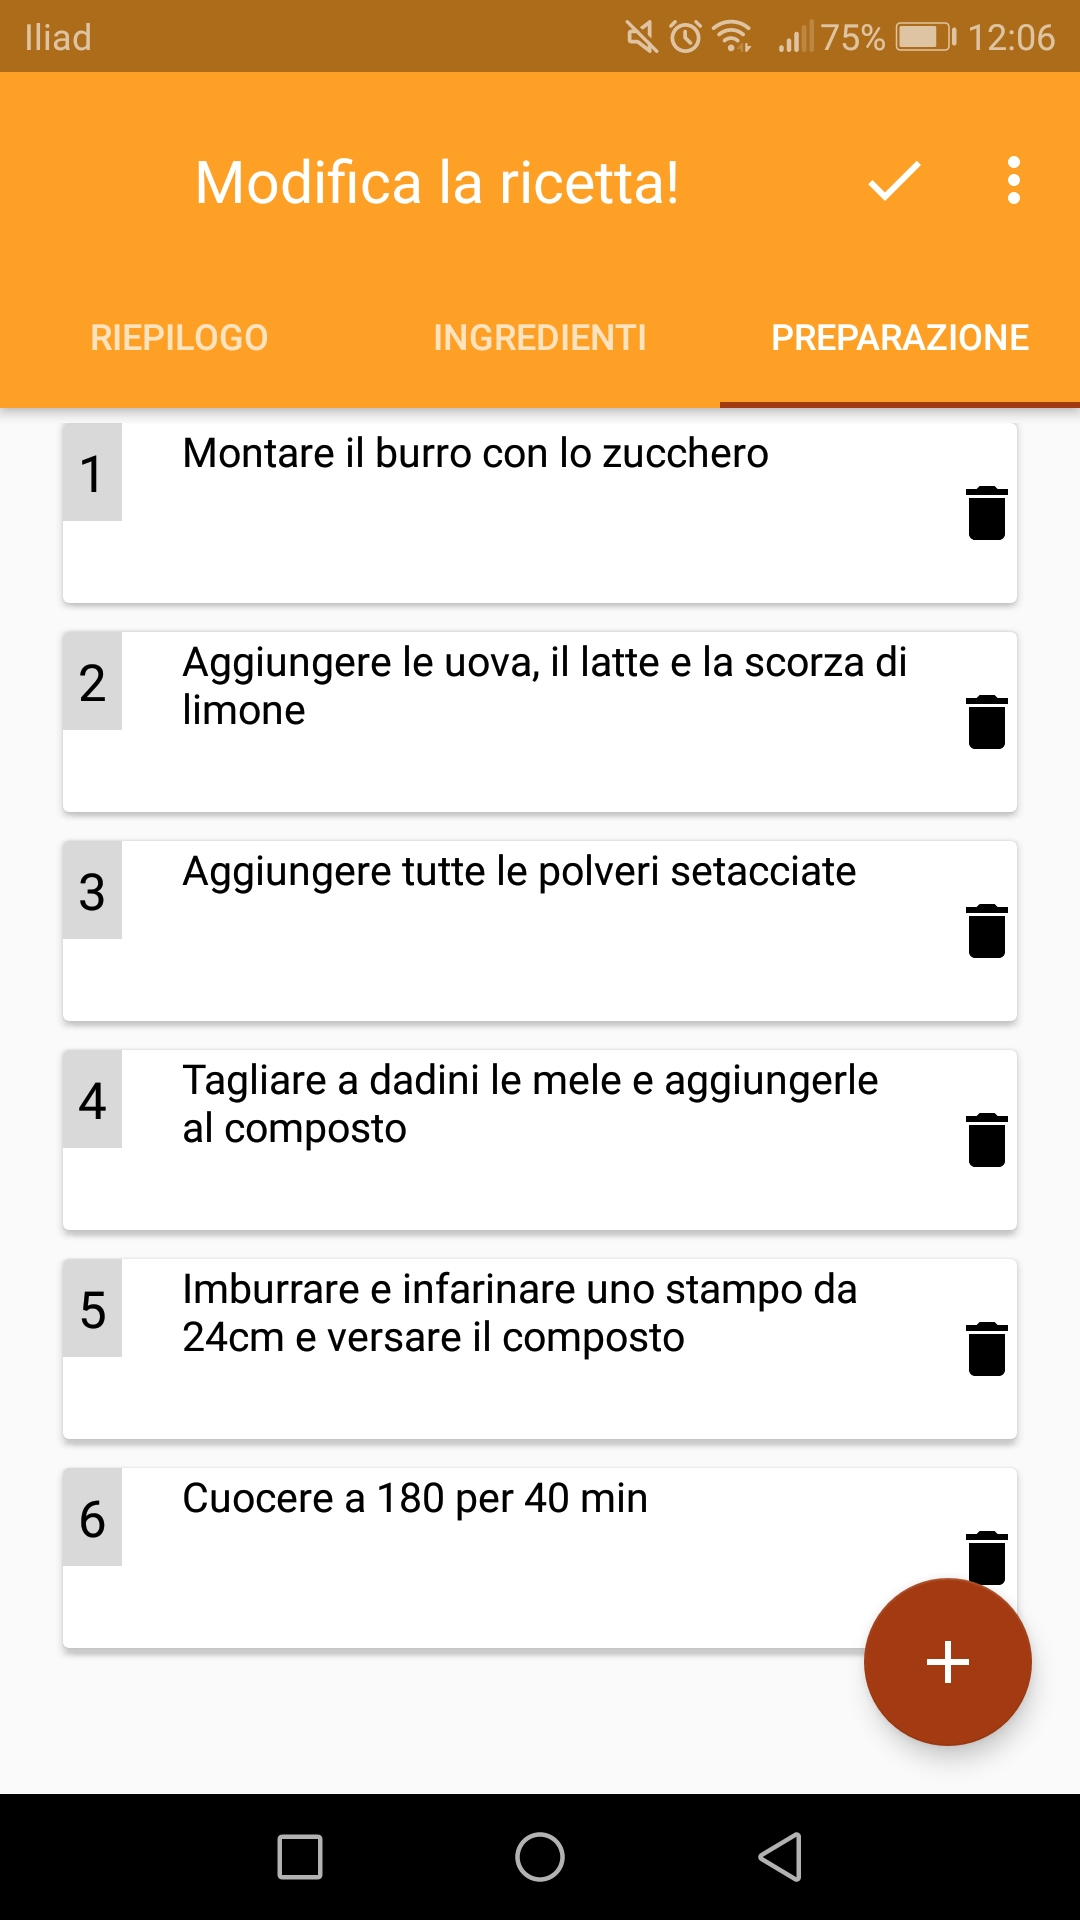
\includegraphics[width=0.49\textwidth]{definitivo/edit_preparazione}
    \caption{Modifica degli ingredienti e dei passaggi}
    \label{fig:def_edit_ricetta}
  \end{center}
\end{figure}

\begin{figure}[ht]
  \begin{center}
    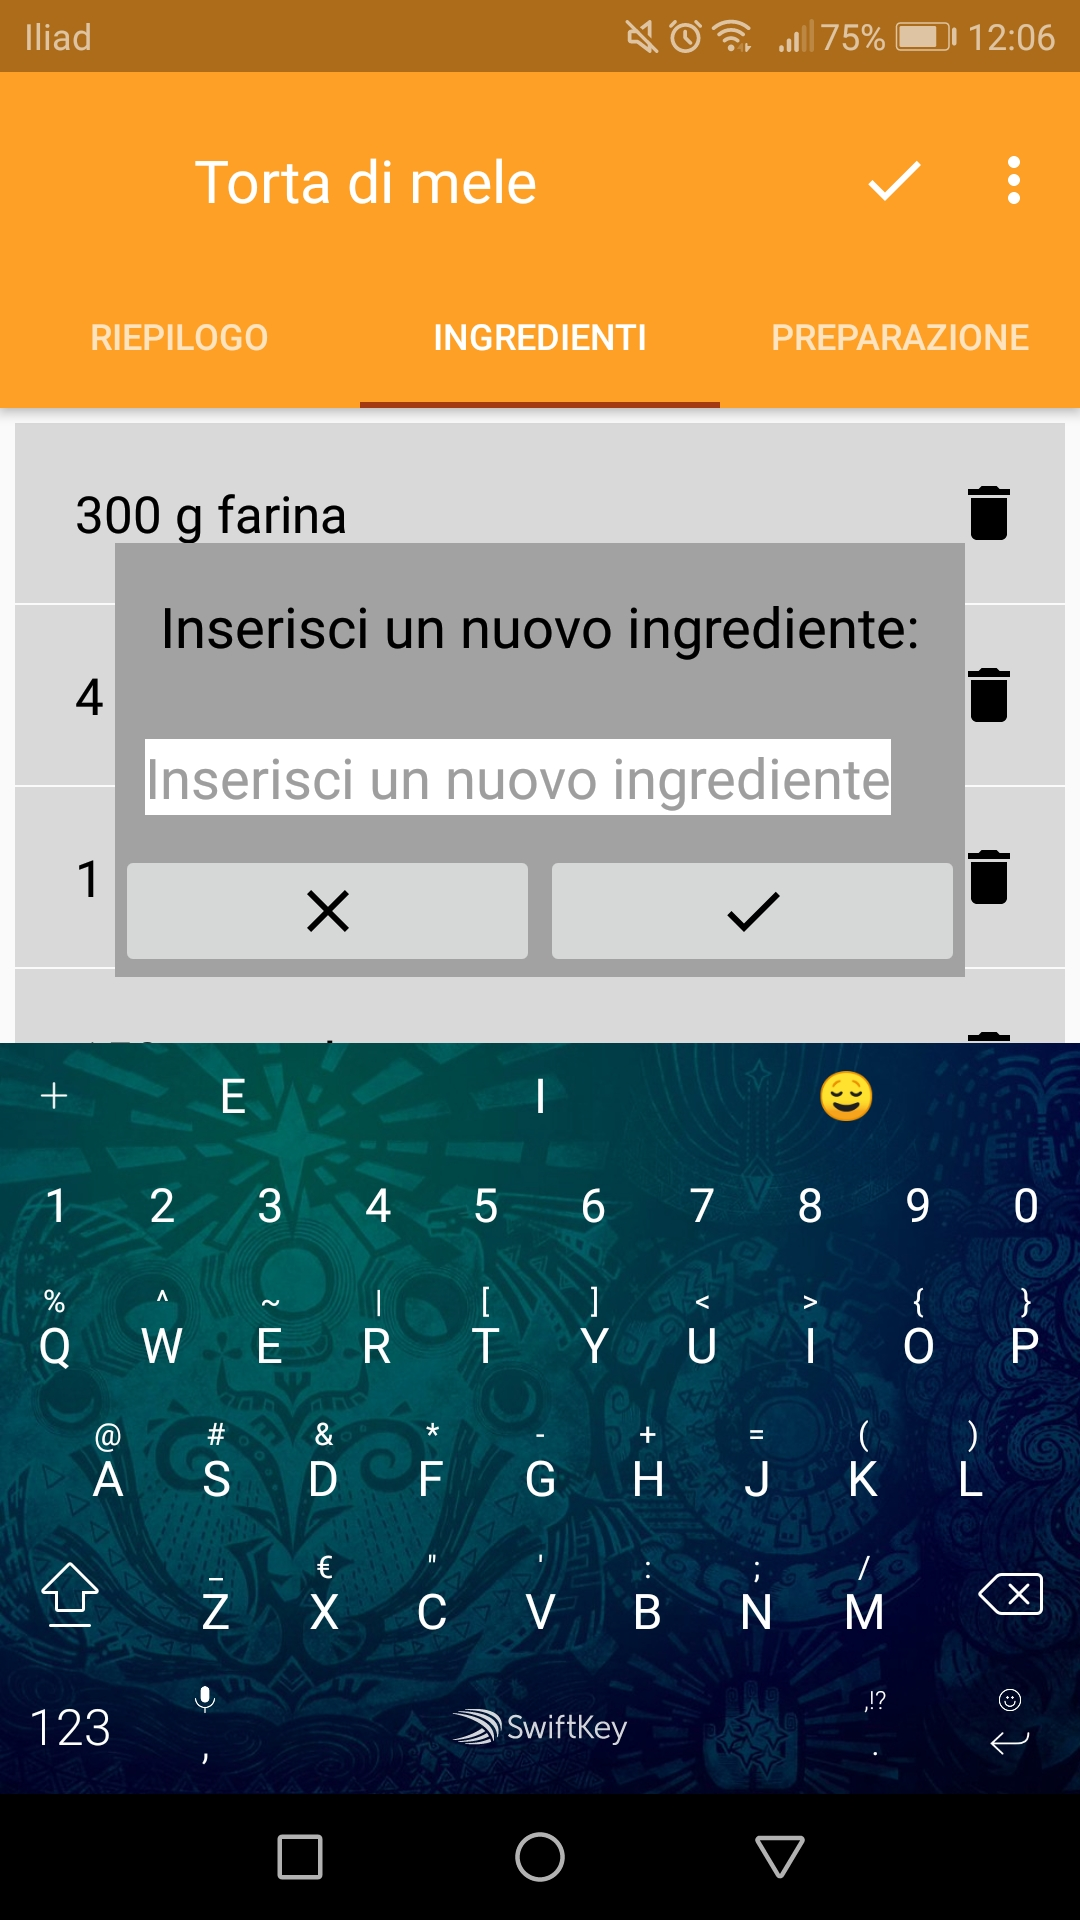
\includegraphics[width=0.49\textwidth]{definitivo/add_ingrediente}
    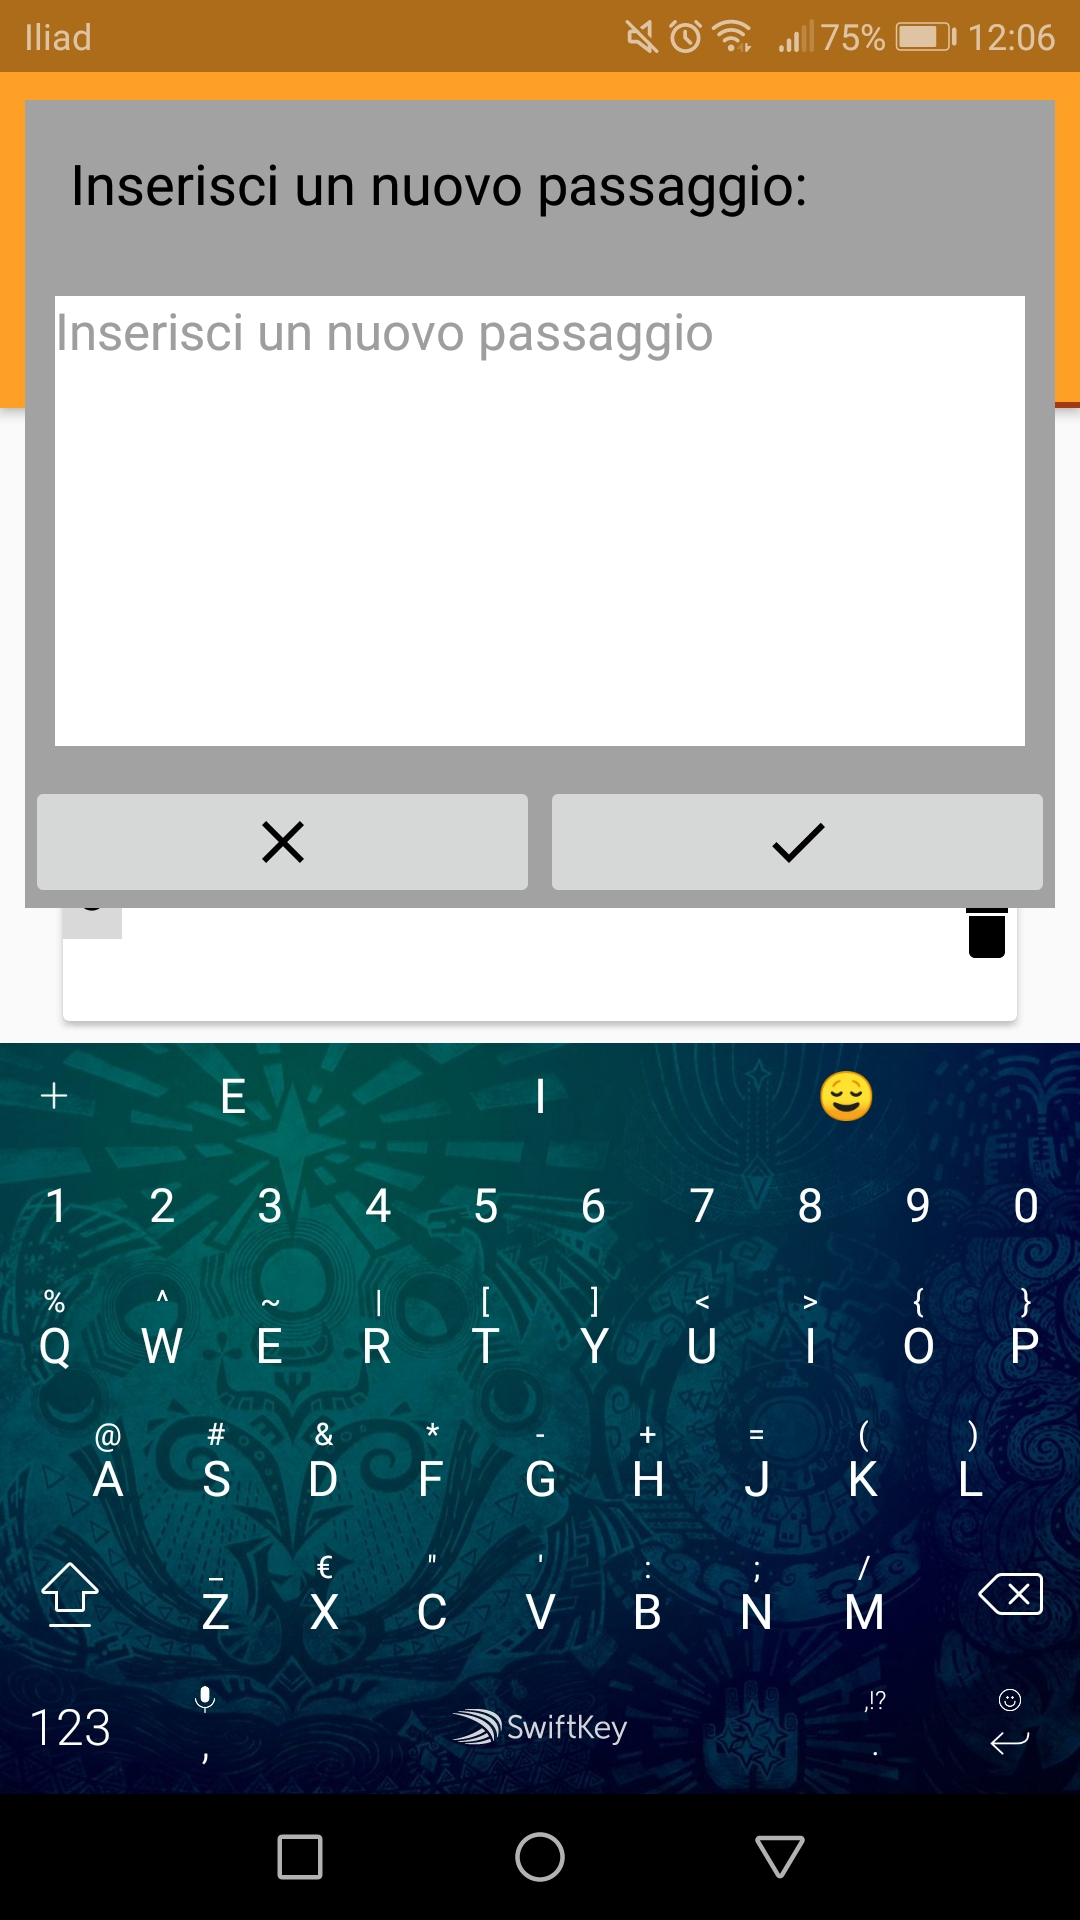
\includegraphics[width=0.49\textwidth]{definitivo/add_step}
    \caption{Finestre di aggiunta ingrediente e passaggio}
    \label{fig:def_edit_ricetta_1}
  \end{center}
\end{figure}

\clearpage
\subsection{Problematiche Principali}
TODO
